% !TEX TS-program = lualatexmk
% glossa-template.tex
% Copyright 2016 Guido Vanden Wyngaerd
%
% This work may be distributed and/or modified under the
% conditions of the LaTeX Project Public License.
% The latest version of this license is in
%   http://www.latex-project.org/lppl.txt
% and version 1.3 or later is part of all distributions of LaTeX
% version 2005/12/01 or later.
%
% This work has the LPPL maintenance status `maintained'.
% 
% The Current Maintainer of this work is 
% Guido Vanden Wyngaerd (guido.vandenwyngaerd@kuleuven.be).
%
% This work consists of the files 
% glossa.cls
% glossa.bst
% gl-authoryear-comp.cbx
% biblatex-gl.bbx
% glossa-template.tex
% glossa.png
%
% The files of the work are derived from the Semantics & Pragmatics style files
% by Kai von Fintel, Christopher Potts, and Chung-chieh Shan
% All changes are documented on the github repository 
% https://github.com/guidovw/Glossalatex.

\PassOptionsToPackage{table}{xcolor}
\PassOptionsToPackage{xcolor}{dvipsnames}
\documentclass[times,linguex,xcolor]{glossa}
\usepackage{rotating}
\usepackage{tablefootnote}
\usepackage{colortbl}
\usepackage{color}
\usepackage{multicol}
\usepackage{booktabs}

\usepackage{adjustbox}
\usepackage{array}

\newcolumntype{R}[2]{%
    >{\adjustbox{angle=#1,lap=\width-(#2)}\bgroup}%
    l%
    <{\egroup}%
}

\newcommand*\rots{\multicolumn{1}{R{90}{.7em}}}% no optional argument here, please!
%\usepackage{xcolor}

% possible options:
% [times] for Times font (default if no option is chosen)
% [cm] for Computer Modern font
% [lucida] for Lucida font (not freely available)
% [brill] open type font, freely downloadable for non-commercial use from http://www.brill.com/about/brill-fonts; requires xetex
% [charis] for CharisSIL font, freely downloadable from http://software.sil.org/charis/
% for the Brill an CharisSIL fonts, you have to use the XeLatex typesetting engine (not pdfLatex)
% for headings, tables, captions, etc., Fira Sans is used: https://www.fontsquirrel.com/fonts/fira-sans
% [biblatex] for using biblatex (the default is natbib, do not load the natbib package in this file, it is loaded automatically via the document class glossa.cls)
% [linguex] loads the linguex example package
% !! a note on the use of linguex: in glossed examples, the third line of the example (the translation) needs to be prefixed with \glt. This is to allow a first line with the name of the language and the source of the example. See example (2) in the text for an illustration.
% !! a note on the use of bibtex: for PhD dissertations to typeset correctly in the references list, the Address field needs to contain the city (for US cities in the format "Santa Cruz, CA")

%\addbibresource{sample.bib}
% the above line is for use with biblatex
% replace this by the name of your bib-file (extension .bib is required)
% comment out if you use natbib/bibtex

\let\B\relax %to resolve a conflict in the definition of these commands between xyling and xunicode (the latter called by fontspec, called by charis)
\let\T\relax
\usepackage{xyling} %for trees; the use of xyling with the CharisSIL font produces poor results in the branches. This problem does not arise with the packages qtree or forest.
%\usepackage[linguistics]{forest} %for nice trees!


% \pdf* commands provide metadata for the PDF output. ASCII characters only!
\pdfauthor{}
\pdftitle{What is at-issueness?}
\pdfkeywords{}

\title[What is at-issueness?]{What is at-issueness? An experimental comparison of diagnostics\\ 
  % \bigskip \large Word count: 4720
  }
% Optional short title inside square brackets, for the running headers.

\author[]% short form of the author names for the running header. If no short author is given, no authors print in the headers.
{%as many authors as you like, each separated by \AND.
  % \spauthor{Waltraud Paul\\
  % \institute{CRLAO, CNRS-EHESS-INALCO}\\
  % \small{%105, Bd. Raspail, 75005 Paris\\
  % waltraud.paul@ehess.fr}
  % }
  % \AND
  % \spauthor{Guido Vanden Wyngaerd \\
  % \institute{KU Leuven}\\
  % \small{%Warmoesberg 26, 1000 Brussel\\
  % guido.vandenwyngaerd@kuleuven.be}
  % }%
}


%=====================================================================
%=========================== text ===========================

	% punctuation
		\usepackage{csquotes} % for quotation marks

%====================================================================
%=========================== links, references =======================
	% more linguex options for referencing select examples without parentheses
	  \newif\ifparens\parensfalse
	  \makeatletter
	  \renewcommand{\theExNo}{\protect\theExLBr\arabic{ExNo}\protect\theExRBr}
	  \renewcommand{\theSubExNo}{%
	    \hbox{\if@noftnote\protect\theExLBr\Exarabic{ExNo}\firstrefdash
	        \Exalph{SubExNo}\protect\theExRBr
	      \else
	        \protect\theFnExLBr\Exroman{FnExNo}\firstrefdash%
	        \Exalph{SubExNo}\protect\theFnExRBr
	      \fi}}

	  \renewcommand{\theSubSubExNo}{%
	    \hbox{\if@noftnote\protect\theExLBr%
	            \Exarabic{ExNo}\firstrefdash\Exalph{SubExNo}\secondrefdash
	               \Exroman{SubSubExNo}\protect\theExRBr%
	      \else\protect\theFnExLBr\Exroman{FnExNo}\firstrefdash
	                \Exalph{SubExNo}\secondrefdash\Exarabic{SubSubExNo}\protect\theFnExRBr\fi}}%
	  \makeatother
	  \renewcommand\theExLBr{\ifparens\else(\fi}
	  \renewcommand\theExRBr{\ifparens\else)\fi}
	  \newcommand\pref[1]{{\parenstrue\ref{#1}}}

	% in text citation macros
	\newcommand{\citepos}[1]{\citeauthor{#1}'s \citeyear{#1}}
	\newcommand{\citeposs}[1]{\citeauthor{#1}'s}
	\newcommand{\citetpos}[1]{\citeauthor{#1}'s \citeyear{#1}}

	%
	\usepackage{cleveref}


%=====================================================================
%=========================== figures, tables =========================
	% \usepackage{subcaption}
	\usepackage{multirow}

% positive coefficients/difference
\definecolor{red}{RGB}{178,24,43}

% negative coefficients/difference
\definecolor{blue}{RGB}{33,102,172}

% comments by JT
\newcommand{\jt}[1]{\textbf{\color{orange}JT: #1}}
\newcommand{\lh}[1]{\textbf{\color{Cerulean}LH: #1}}

\begin{document}


\maketitle


\begin{abstract}
  at-issueness is a key concept in theoretical semantics/pragmatics, but there is no consensus about how it is defined or diagnosed (e.g., \citealt{tonhauser_diagnosing_2012,snider_anaphoric_2017,snider_distinguishing_2018,tonhauser_how_2018,koev_notions_2018,faller_discourse_2019,korotkova_evidential_2020}). We present experimental data investigating whether four widely used diagnostics for at-issueness yield consistent results. Our findings reveal significant differences across diagnostics, indicating they are not interchangeable. Since the diagnostics target distinct theoretical conceptions of at-issueness, these differences offer insight into their comparability.

\end{abstract}

% \begin{keywords}
%   at-issueness, experimental pragmatics, discourse interpretation
% \end{keywords}

\section{Introduction \label{sec:1_introduction}}
  
  At-issueness is a key concept in theoretical semantics and pragmatics, used in the analysis of a wide range of phenomena, including presupposition, conventional implicature, evidentials, expressives, and NPI licensing (e.g., \citealt{karttunen_conventional_1979,horton_presuppositions_1988,abbott_presuppositions_2000,faller_semantics_2003,potts_logic_2005,tonhauser_diagnosing_2012,horn_licensing_2016}). Although at-issuness is widely understood as distinguishing propositions expressing the main point of an utterance (at-issue content) from those conveying background information (not-at-issue content), there is no consensus on how to define this distinction. Multiple competing definitions and diagnostics exist, each grounded in different assumptions about the nature of the distinction.

  Four commonly used diagnostics are illustrated in (\pref{qud}--\pref{yesbut}) for sentence-medial appositive non-restrictive relative clauses (NRRCs), which are typically taken to contribute not-at-issue content (\citealt{potts_logic_2005}). Accordingly, participants are expected to: give low question-answer-match ratings under the QUD diagnostic \ref{qud}; not interpret the speaker to be asking about the NRRC content under the `asking-whether' diagnostic \ref{aw}; give low naturalness ratings under the direct-dissent diagnostic \ref{dd}; and prefer a \emph{yes}-response under the `yes, but' diagnostic in \ref{yesbut}.

  \ex. \label{qud}%
    QUD diagnostic (e.g., \citealt{tonhauser_diagnosing_2012,chen_presuppositions_2024})
    \a.[A:] \emph{What did Greg buy?}
    \b.[B:] \emph{Greg, who bought a new car, is envied by his neighbor.}
    \z.
    Question to participants: How well does B's response fit A's question?
  \z.

  \ex. \label{aw}%
    `asking whether' diagnostic (e.g., \citealt{tonhauser_how_2018,solstad_cataphoric_2024})\smallskip\\
      \emph{Is Greg, who bought a new car, envied by his neighbor?}\smallskip
  \\ Question to participants: Is the speaker asking whether Greg bought a new car?
  \z.

  \ex. \label{dd} Direct dissent diagnostic (e.g., \citealt{tonhauser_diagnosing_2012,syrett_experimental_2015})
    \a.[A:] \emph{Greg, who bought a new car, is envied by his neighbor.}
    \b.[B:]\emph{No, that's not true, he didn't buy a new car.}
    \z.
  Question to participants: How natural is B's rejection of A's utterance?
  \z.

  \ex. \label{yesbut}%
    `yes, but' diagnostic (e.g., \citealt{xue_correlation_2011,destruel_cross-linguistic_2015})
    \a.[A:] \emph{Greg, who bought a new car, is envied by his neighbor.}
    \b.[B:] \emph{Yes, but he didn't buy a new car.} /
    \b.[] \emph{Yes, and he didn't buy a new car.} /
    \b.[] \emph{No, he didn't buy a new car.}
    \z.
    Task for participants: Choose the response that sounds best.
  \z.

  The QUD diagnostic \ref{qud} and the ‘asking-whether’ diagnostic \ref{aw} assume that discourse is structured around addressing a question under discussion (QUD, \citealt{roberts_information_1996,ginzburg_interrogatives_1996}), and that at-issue content is the part of an utterance that interacts with the current QUD (\citealt{amaral_review_2007,simons_what_2010}). Specifically, the QUD diagnostic (\citealt{tonhauser_diagnosing_2012}) assumes that only at-issue content can respond to a QUD established in prior discourse, and the `asking whether' diagnostic (\citealt{tonhauser_how_2018}) assumes that the at-issue content of questions explicitly raises a QUD, whereas their not-at-issue content does not contribute to what the QUD is.

  Research about at-issueness diagnostics has pointed out that the assumptions behind the question-based diagnostics are quite different from the the assent/dissent-based diagnostics (\pref{dd}+\pref{yesbut}), which are not usually interpreted within a QUD-framework (\citealt{snider_anaphoric_2017,snider_at-issuenessne_2017,snider_distinguishing_2018,koev_notions_2018,faller_discourse_2019,korotkova_evidential_2020}).
  %
  Snider argues that the latter kind of diagnostics may not reflect at-issueness at all, but rather target the anaphoric availability of propositional content for response particles (e.g., English \emph{yes/no}).
  %
  On another view, these diagnostics target a distinct notion of at-issueness (see \citealt{koev_notions_2018} and discussion in \citealt{faller_discourse_2019,korotkova_evidential_2020}), under which the at-issue content of an assertion constitues a proposal to update the common ground (based on \citealt{farkas_reacting_2010}). Accordingly such content can be directly affirmed or denied using default discourse moves that include response particles. Conversely, not-at-issue content is either presupposed (already entailed in the common ground; \citealt{stalnaker_presuppositions_1973,stalnaker_common_2002}), or newly imposed on the common ground (\citealt{murray_varieties_2014,anderbois_at-issue_2015}), and requires special discourse moves for rejection (\citealt{potts_logic_2005}).

  Consequently, we are currently faced with a landscape where there is no agreed-upon definition of at-issueness and where different diagnostics may not be tapping into the same underlying phenomenon. This raises two critical questions:

  \begin{enumerate}
    \item Do the various diagnostics yield the same results?
    \item Do the existing definitions of at-issueness describe the same underlying phenomenon?
  \end{enumerate}

  \noindent Some research has suggested that the answers to both of these questions may be ``no''.

  On the empirical side, the often reported tendency for adnominal appositives to contribute not-at-issue content (following \citealt{potts_logic_2005}) is supported by several studies, however, findings vary based on their position in the sentence (sentence-medial or sentence-final) and which diagnostic is used:
  %
  Under the direct-dissent test, medial appositives consistently behave as not-at-issue across multiple languages and methods, including fieldwork elicitation for Paraguayan Guaraní (\citealt{tonhauser_diagnosing_2012}), an English forced-choice continuation task (\citealt{syrett_experimental_2015}), and impressionistic English judgments (\citealt{potts_logic_2005,amaral_review_2007}). Similar patterns emerge from an experimental study using the `yes, but' diagnostic in German (\citealt{destruel_cross-linguistic_2015}), and the `asking whether' diagnostic (\citealt{tonhauser_how_2018,solstad_cataphoric_2024} with English and German stimuli, respectively). All of these studies find that medial appositives tend to receive more ratings that indicate a not-at-issue status.\footnote{
      Whether appositives can address the QUD is contested. 
      %
      For English medial appositive NRRCs, though not-at-issue under the direct-dissent test, it has been argued that they can behave as at-issue under the QUD diagnostic in a handful of examples (\citealt{anderbois_at-issue_2015,syrett_experimental_2015}).
      %
      This is consistent with \citepos{tonhauser_diagnosing_2012} findings for Paraguayan Guaraní medial appositive DPs: These are not-at-issue on most diagnostics tested there (including direct dissent, and `yes, but'), but yielded mixed results with the QUD-diagnostic.

      \citealt{snider_anaphoric_2017} counters that the sporadic examples used as evidence that English medial appositives can be at-issue under the QUD-diagnostic involve a misapplication of the diagnostic (p.256--258).
      %
      A finding from \citealt{chen_presuppositions_2024} could be interpreted as supporting this view. Her findings from (the adults in) Experiment 1 show relatively low QUD-match ratings for German medial NRRCs; however, these clauses also contained the discourse marker \emph{übrigens} (‘by the way’), which, Chen suggests, itself cues a not-at-issue reading.
      
    }

  In contrast, it has been argued that sentence-final appositive NRRCs can be interpreted as at-issue, based on findings from the direct-dissent diagnostic, for instance, using English corpus examples in \citealt{anderbois_at-issue_2015}, and notably \citepos{syrett_experimental_2015} forced-choice continuation task experiment.

  Theoretically, \citepos{syrett_experimental_2015} main finding, that final appositive NRRCs receive more `yes but' responses than medial ones has received three main interpretations:
  \begin{enumerate}

    \item Final appositives are more at-issue than medial ones at the point in discourse when participants choose a response (\citealt{syrett_experimental_2015,jasinskaja_not_2016}).

    \item Medial and final appositives are both not-at-issue, and rather than diagnosing at-issueness, the direct-dissent diagnostic diagnoses anaphoric availabiltiy, which is a distinct notion that is affected by factors like recency (\citealt{snider_anaphoric_2017,snider_at-issuenessne_2017,snider_distinguishing_2018}).

    \item  A final appositive cannot address the QUD, but it is part of the asserted content; so we are dealing with two distinct notions of at-issueness (a second option considered by \citet{snider_anaphoric_2017}, see also discussion in \citealt{koev_notions_2018}).

  \end{enumerate}

  Beyond adnominal appositives, \citealt{tonhauser_how_2018} compared at-issueness measures for a range of 19 English expressions (including appositives, expressions that are usually characterized as presupposition triggers, and clause-embedding predicates), using two diagnostics: the question-based `asking whether' diagnostic and the `Are you sure?' diagnostic (p.526ff). They found that contents generally received higher not-at-issueness ratings with the `asking whether' diagnostic, while the `Are you sure?' diagnostic showed greater variability both within and across expressions. Despite these differences, ratings from both diagnostics correlated with measures of projection inferences, suggesting that the two diagnostics may, in fact, be sensitive to a shared underlying phenomenon.


  \bigskip \hrule\bigskip
  On the diagnostics-side, Tonhauser et al 2018 asking whether didn’t find difference in exp 1a between know and discover (see also Solstad/Bott) but Xue/Onea found difference between wissen and entdecken

  \begin{itemize}
    \item Using the `asking whether' diagnostic, 
    \item  Tonhauser et al. 2018 observed differences between sentence-final NRRCs and the contents of the complements of know, discover and confess using the ‘asking whether’ diagnostic

    \item Using a slider reponse task, \citealt{tonhauser_how_2018} found that clauses embedded under \emph{know} and \emph{discover} are clearly not-at-issue,\jt{really? i mean, we didn't run stats but looking at the figure and the means, is this really so clear? the CC of discover is less not-at-issue than the content of NRRCs. i'd like to move away from a binary talk about at-issueness.} and those under \emph{confess} only slightly less so.

    \item Tonhauser et al 2018 asking whether didn't find difference in exp 1a between know and discover (see also Solstad/Bott) but Xue/Onea found difference between wissen and entdecken

    However, \citealt{solstad_cataphoric_2024} finds that the embedded contents of German \emph{wissen} `know' and \emph{entdecken} `discover' are interpreted as not-at-issue, using `asking whether' diagnostic and the same methodology as \citealt{tonhauser_how_2018,degen-tonhauser-glossa}.

  \end{itemize}

  Further, Degen/Tonhauser 2025 found fine-grained differences between CCs of clause-embedding predicates using the asking-whether diagnostic, where Hooper 1975 distinguished weak assertive (e.g., think, acknowledge), strong assertive (e.g., say, suggest), semi-factive (assertive; e.g., see, discover, know) and factive (nonassertive; e.g., be annoyed).

  \begin{itemize}
    \item Using the `asking whether' diagnostic, \citealt{degen-tonhauser-glossa} found fine-grained lexical differences for the at-issueness of the embedded content of 20 English clause-embedding predicates: \Cref{fig:dtglossa} shows the distribution of `asking whether' ratings by predicate with means and 95\% bootstrapped confidence intervals. Their results again place the complement of \emph{know} solidly in the not-at-issue range,\jt{this sounds like there's a not-at-issue range and an at-issue range?} while \emph{discover} and \emph{confess}, with mean ratings around $0.6$ on the 0--1 scale, show only a weak preference towards a not-at-issue interpretation.

  \end{itemize}

  
  \begin{figure}[h!]
    \centering

    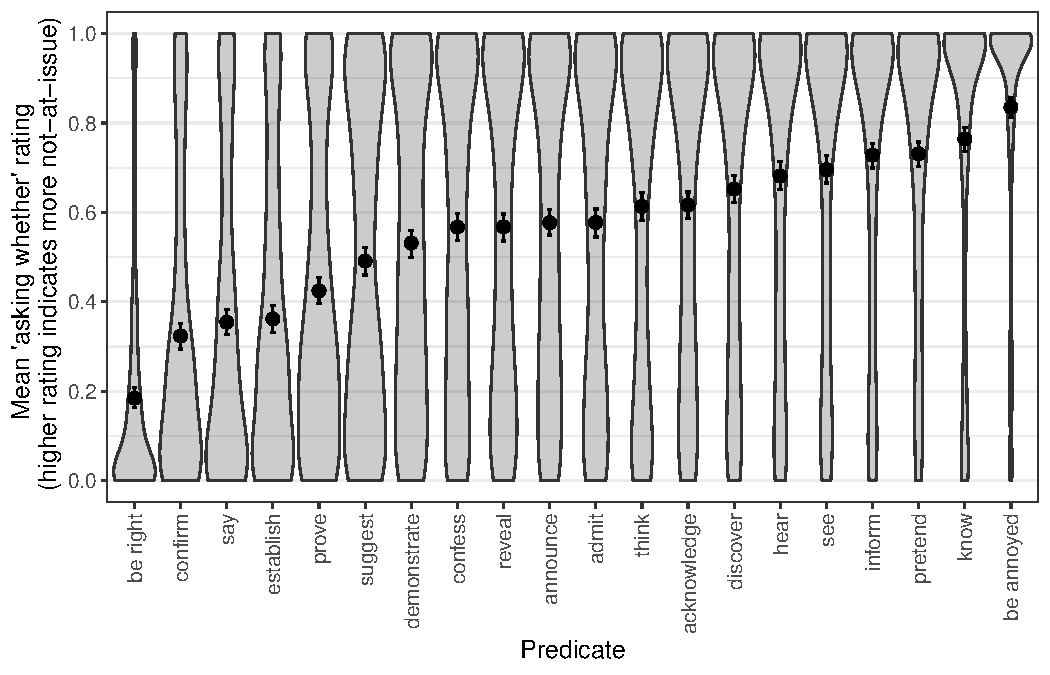
\includegraphics[width=0.7\textwidth]{../../results/degen-tonhauser-glossa/graphs/mean-asking-whether-ratings.pdf}

    \caption{Mean `asking whether' ratings for the contents of the clausal complements of 20 clause-embedding predicates, from \citealt{degen-tonhauser-glossa}.}
    \label{fig:dtglossa}
  \end{figure}
  
  \bigskip \hrule\bigskip


  To date, there has been no systematic comparison of diagnostics to investigate whether they yield consistent results about at-issueness.
  This paper takes a first step toward addressing the above questions (i+ii) in a systematic way. Specifically, we assess whether the four widely used diagnostics in (\pref{qud}--\pref{yesbut}) give rise to the same pattern of results when applied to the same target contents. Our findings reveal significant differences across diagnostics, indicating they are not interchangeable. Because each diagnostic is underpinned by distinct theoretical assumptions about what it means for content to be at-issue, this comparison also speaks to the question of whether currently available conceptions of at-issueness converge on a common underlying notion.

  We present the results from a series of experiments that systematically vary the diagnostic used to assess the at-issueness status of the same types of contents across experiments. Experiments 1--4 tests sentence-medial and sentence-final NRRCs, and the embedded complements of selected clause-embedding predicates. These contents were selected because previous research has found variability in their behavior on at-issueness diagnostics:
  \begin{itemize}
    \item medial and final NRRCs yield different results on the direct dissent diagnostic (e.g., \citealt{syrett_experimental_2015}), while differing clause-embedding predicates have been shown to yield fine-grained differences in at-issueness measures (e.g., \citealt{tonhauser_how_2018,degen-tonhauser-glossa}).
    \item relate to empirical discussion above (selection of contents)
    \item Are these differences between contents replicated by the use of other diagnostics? (also relate)
  \end{itemize}

  In experiments 5 and 6, we test whether the fine-grained differences among clause-embedding predicates observed with one diagnostic (asking-whether) are replicated with other diagnostics.
  \begin{itemize}
    \item CCs of clause-embedding predicates because one diagnostic found fine-grained differences
    \item Are these differences between contents replicated by the use of other diagnostics?
  \end{itemize}
  
  By directly comparing how these contents are evaluated by each diagnostic, our study provides the first thorough assessment of the comparability and interchangeability of at-issueness diagnostics.

  \bigskip \hrule\bigskip

  In this paper, we operationalize each diagnostic through its established empirical task: question-answer match ratings for the QUD diagnostic, speaker intention judgments for the asking-whether diagnostic, naturalness ratings for direct dissent, and forced-choice responses for the ‘yes, but’ diagnostic.

  For each of the contents, we collect ratings across multiple items and participants, and compare the mean responses. Given that we are aggregating over multiple items and participants
  % (and ratings on a scale for some),
  we may say that the mean rating for one content is higher/lower than that of another, or that they do not differ. Following prior work (e.g., \citealt{tonhauser_how_2018}), we interpret higher mean/lower ratings as indicating that content is more/less at-issue under a given diagnostic, with two caveats:

  First, we remain agnostic about whether at-issueness is an underlyingly binary or a gradient property (cf. \citealt{tonhauser_how_2018,barnes_information_2023}). If at-issueness is gradient, the extent to which content is at-issue of a content may be understood as the extent to which it is relevant to the QUD or the main assertion, in which case gradient mean ratings may be taken to reflect gradient relevance. If at-issueness is categorical, content is at-issue iff it addresses the QUD or assertive proposal, and not-at-issue otherwise; and gradient mean ratings could be attributed to uncertainty about what the QUD is. For example, our interpretation of a content in a given utterance being more/less at-issue may be interpreted as reflecting the frequency or ease with which a particular QUD is attributed to that utterance.

  Second, we use the term “at-issueness diagnostic” descriptively throughout the paper, even though our findings may ultimately suggest that these diagnostics track distinct theoretical constructs. We return to this issue in the general discussion.


\bigskip

\noindent
{\bf Bigger story of the paper}

  \begin{itemize}[leftmargin=12pt]

  \item Exps 1-4 suggest than none of the diagnostics as implemented distinguish between sentence-medial and -final NRRCs, not even the `direct dissent' diagnostic of Exp 3, contra Syrett/Koev. 

  \item This suggests that even small changes like the response task might matter and also that the diagnostics differ in whether they predict a differences in at-issueness between sentence-medial and -final NRRCs.

  \item Of Exps 1-4, only Exp 2 (asking whether) comes close to suggesting the difference in the CCs of the clause-embedding predicates observed in Degen/Tonhauser 2025. This suggests that the diagnostics differ in whether they predict a differences in at-issueness between the CCs of clause-embedding predicates.

  \item Overall, Exps 1-4 suggest that at-issueness diagnostics are not interchangeable as they differ in the relative differentiation of the seven contents investigated. 

  \item Given that the diagnostics pertain to different definitions of at-issueness, this also suggests that those definitions may define different concepts; as suggested in Snider.

  \item {\bf Discussion of section 2:} The asking-whether diagnostic shows the greatest differentiation between the contents.  It is the only diagnostic where the contents to be diagnosed are in polar interrogatives and the diagnostic relies on the assumption that at-issue content partitions the context set denoted by the polar interrogative.

  \item Question: Is the differentiation due to the content being embedded in an interrogative or due to the response task (which is about which content partitions the context set)?

  \item Exps 5-6: We investigate the aforementioned question by comparing asking whether diagnostic (Exp 5) to direct assent diagnostic where content is embedded in interrogative (Exp 5)

  \item We find high correlation (Spearman rank), so this suggests that the high differentiation may be due to interrogative embedding and not the response task (partition of context set by at-issue content). 

  \item {\bf General discussion:} 

  \begin{itemize}

  \item diagnostics give different results; some of these differences may be due to response tasks, others may be due to different underlying concepts

  \item interrogative embedding seems to matter, so speech acts also need to be taken into consideration when considering what at-issueness is and how it is diagnosed

  \item future research will need to make sure that results may only be due to particular response task used, empirical investigations should continue path of using multiple diagnostics 

  \end{itemize}

  \end{itemize}


    
  \newpage


\section{Experiments 1-4 \label{sec:2_experiments}}

  To compare the results of at-issueness diagnostics, we conducted four experiments that each measured at-issueness with a different diagnostic, namely the QUD diagnostic (Exp.~1), the `asking whether' diagnostic (Exp.~2), the direct-dissent diagnostic (Exp.~3) and the `yes, but' diagnostic (Exp.~4).\footnote{The experiments, data and R code for generating the figures and analyses of the experiments reported in this paper are available at INSERT URL TO ANONYMOUS GITHUB REPO BEFORE SUBMISSION. All experiments were conducted with approval from the ethics review committee of [university name redacted for review]. \label{f:github}}
  Each experiment itested the same manipulation, comparing seven types of contents, introduced by the embeddings shown in \ref{stims}: the contents of sentence-medial and sentence-final NRRCs \ref{stims.a}-\ref{stims.b}, as well as the contents of the clausal complements of \emph{know, discover, confess, confirm} and \emph{be right} \ref{stims.c}-\ref{stims.g}. These seven contents were randomly paired with one from a set of items shared across all four experiments.

  \ex.\label{stims}
    \a.\label{stims.a} Content of sentence-medial NRRC \\
      \emph{Lucy, who broke the plate, apologised.} $\leadsto$ Lucy broke the plate
    \b.\label{stims.b} Content of sentence-final NRRC \\
    \emph{The police found Jack, who saw the murder.} $\leadsto$ Jack saw the murder
    \b.\label{stims.c} Content of the clausal complement of \emph{know} \\
    \emph{Ann knows that Raul cheated on his wife.} $\leadsto$ Raul cheated on his wife
    \b.\label{stims.d} Content of the clausal complement of \emph{discover} \\
    \emph{Mary discovered that Denny ate the last cupcake.} $\leadsto$ Denny ate the last cupcake
    \b.\label{stims.e} Content of the clausal complement of \emph{be right} \\
    \emph{Tom is right that Ann stole the money.} $\leadsto$ Ann stole the money
    \b.\label{stims.f} Content of the clausal complement of \emph{confirm} \\
    \emph{Harry confirmed that Greg bought a new car.} $\leadsto$ Greg bought a new car
    \b.\label{stims.g} Content of the clausal complement of \emph{confess}  \\
    \emph{Lucy confessed that Dustin lost his key.} $\leadsto$ Dustin lost his keys
    \z.
  \z.

  These seven contents were chosen because prior literature observed differences in at-issueness between two or more of these contents using a particular diagnostic for at-issueness.  Specifically, as discussed in \S1, \citealt{syrett_experimental_2015} observed differences between sentence-medial and -final NRRCs using a variant of the direct-dissent diagnostic, \citealt{tonhauser_how_2018} observed differences between sentence-final NRRCs and the contents of the complements of \emph{know, discover} and \emph{confess} using the `asking whether' diagnostic, and \citealt{degen-tonhauser-glossa} observed differences between \emph{know, discover, confess, confirm} and \emph{be right}, also using the `asking whether' diagnostic. Thus, comparing these seven contents across the four diagnostics in Exps.~1-4 will allow us to assess whether the differences that emerge from one diagnostic also emerge from others. In each experiment, participants read the stimuli and gave ratings corresponding to the diagnostics.

  \subsection{Methods}
    
  \subsubsection{Participants}

  For each of the four experiments, we recruited 80 unique participants on Prolific. These participants had registered on the platform as living in the USA and as having English as their primary language. They had at least 50 previous submissions and an approval rate of at least 97\%.  Table \ref{t:recruited} shows the age and gender distributions of the recruited participants.

  \begin{table}[h!]
  \centering
  \begin{tabular}{l | c | r r r }
              & recruited & ages (mean age) & f/m/nb/dnd \\ \hline
  Exp.~1 (QUD) & 80 & 18-81 (43.8) & 42/37/0/1  \\
  Exp.~2 (asking whether) & 80 & 20-74 (38.5)  & 48/30/1/1  \\
  Exp.~3 (direct dissent) & 80 & 18-77 (39.1) & 50/28/1/1  \\
  Exp.~4 (yes, but) &80 & 19-67 (38.0)  & 48/30/2/0 &  \\
  \hline
  \end{tabular}

  \caption{Information about the participants recruited in Exps.~1-4 (f = female, m = male, nb = nonbinary, dnd = did not disclose).}\label{t:recruited}
  \end{table}

  \subsubsection{Materials and procedure}
  
  The four experiments measured the at-issueness of the seven contents in \ref{stims} with a different at-issueness diagnostic, namely the QUD diagnostic (Exp.~1), the `asking whether' diagnostic (Exp.~2), the direct-dissent diagnostic (Exp.~3) and the `yes, but' diagnostic (Exp.~4). The examples in \ref{diag} illustrate how each diagnostic was implemented using the content of sentence-medial NRRCs (with the item `Lucy broke the plate'). In Exp.~1 (QUD diagnostic, \ref{diag.a}), participants read a dialogue between two named speakers, where the first utters an interrogative sentence (the presumed QUD) that is about the content to be diagnosed and the second responds with a declarative sentence that contributes the content to be diagnosed. In Exp.~2 (`asking whether' diagnostic, \ref{diag.b}), participants read an interrogative sentence uttered by a named speaker, where the interrogative sentence contributes the content to be diagnosed. In Exp.~3 (`direct dissent' diagnostic, \ref{diag.c}), participants read a dialogue between two named speakers, where the first utters a declarative sentence with the content to be diagnosed and the second directly dissents with the content to be diagnosed. Finally, in Exp.~4 (`yes, but' diagnostic, \ref{diag.d}), participants read a dialogue between two named speakers where the first utters a declarative sentence that contributes the content to be diagnosed and the second responds with one of two indirect dissent variants (\emph{yes, but..}, \emph{yes, and...}) or with a direct dissent.

  \ex.\label{diag} Implementations of the diagnostics in Exps.~1-4
  \a.\label{diag.a} Exp.~1 (QUD diagnostic)
  \\ {\bf Nora:} \emph{What did Lucy break?}
  \\ {\bf Leo:} \emph{Lucy, who broke the plate, apologized.}
  \b.\label{diag.b} Exp.~2 (`asking whether' diagnostic )
  \\ {\bf Nora:} \emph{Did Lucy, who broke the plate, apologize?}
  \c.\label{diag.c} Exp.~3 (`direct dissent' diagnostic)
  \\ {\bf Nora:} \emph{Lucy, who broke the plate, apologized.}
  \\ {\bf Leo:} \emph{No, she didn't break the plate.}
  \d.\label{diag.d} Exp.~4 (`yes, but' diagnostic)
  \\ {\bf Nora:} \emph{Lucy, who broke the plate, apologized.}
  \\ {\bf Nina:} \emph{Yes, but she didn't break the plate.}
  \\ \hspace*{1cm} \emph{Yes, and she didn't break the plate.}
  \\ \hspace*{1cm} \emph{No, she didn't break the plate.}



  As shown in Fig.~\ref{fig:trials}, the response options in each of the four experiments differed depending on the diagnostic. In Exp.~1 (QUD diagnostic, panel (a)), participants were asked how well the response fits the question and they gave their response on a slider marked `totally doesn't fit' on one end (coded 0) and `totally fits' on the other end (coded as 1). In Exp.~2 (`asking whether' diagnostic, panel (b)), participants were asked whether the question is about the content to be diagnosed and they gave their response on a slider marked `no' on one end (coded as 1) and `yes' on the other (coded as 0). In Exp.~3 (direct-dissent diagnostic, panel (c)), participants were asked how natural the direct dissent and participants gave their response on a slider marked `totally unnatural' (coded as 0) on one end and `totally natural' on the other (coded as 1). Finally, in Exp.~4 (`yes, but' diagnostic, panel (d)), participants were asked to choose the response that sounded best; the two indirect dissents were coded as 1 and the direct one as 0. Across the four experiments, the responses were coded as 0 or 1 in such a way that 0 meant that the content to be diagnosed was rated as at-issue and 1 meant that the content was rated as not-at-issue.

  \lh{I find the scale-reversal confusing, especially in Exp. 1 and 3, I find it counterintuitive in relation to the acceptability rating tasks there. What is the benefit of reversing the scale? (I dont really see it...) Maybe we could keep the non-reversed version here? I think that this will actually really help in the discussion of how much the diagnostics reflect at-issueness, to say things in a more intuitive way, when there are independent facors that affect the aceptability ratings beyond at-issueness.}


 \begin{figure}[h!]
  \centering
  % Top row
  \subfigure[Exp.~1: QUD diagnostic]{%
    \fbox{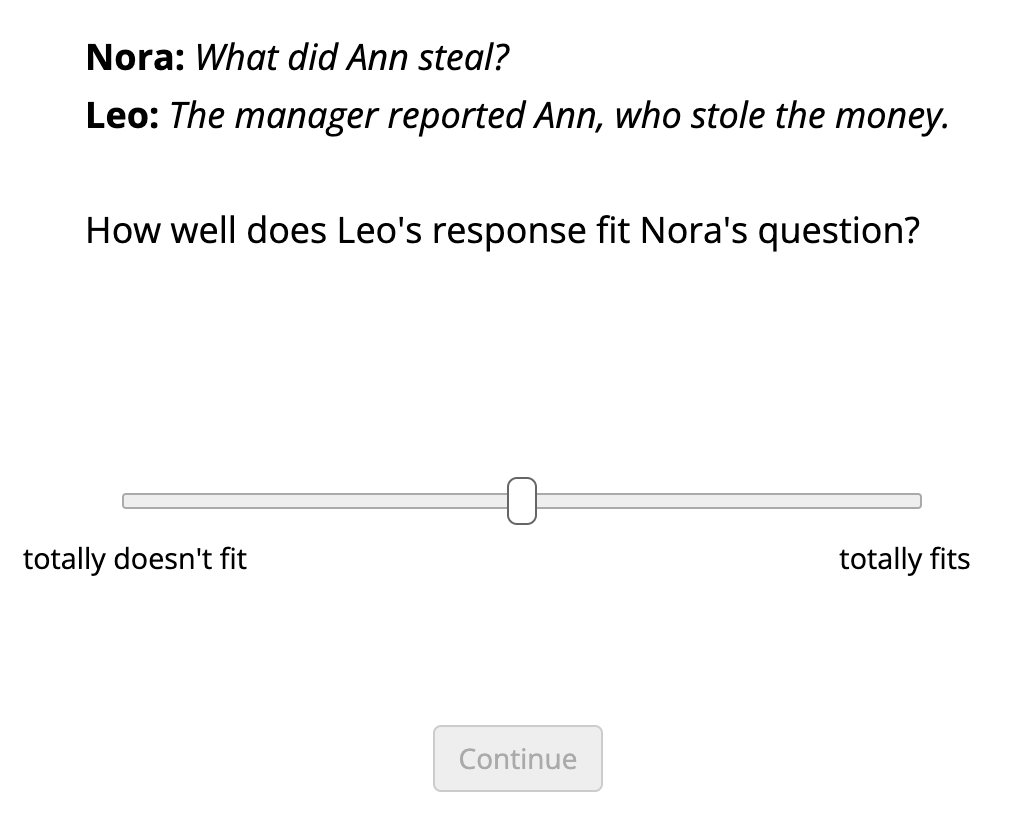
\includegraphics[width=0.47\textwidth]{figures/trialExp1}}%
    \label{fig:trialExp1}
  }
  \hfill
  \subfigure[Exp.~2: `asking whether' diagnostic]{%
    \fbox{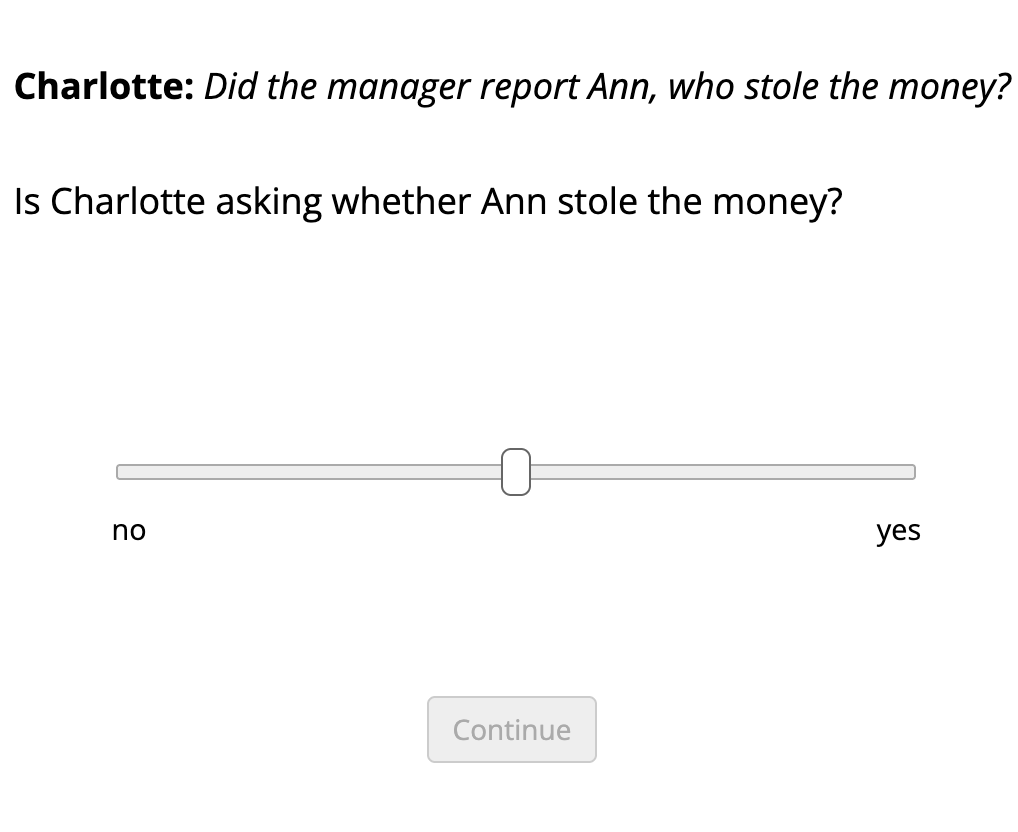
\includegraphics[width=0.47\textwidth]{figures/trialExp2}}%
    \label{fig:trialExp2}
  }

  \vspace{1em}

  % Bottom row
  \subfigure[Exp.~3: `direct dissent' diagnostic]{%
    \fbox{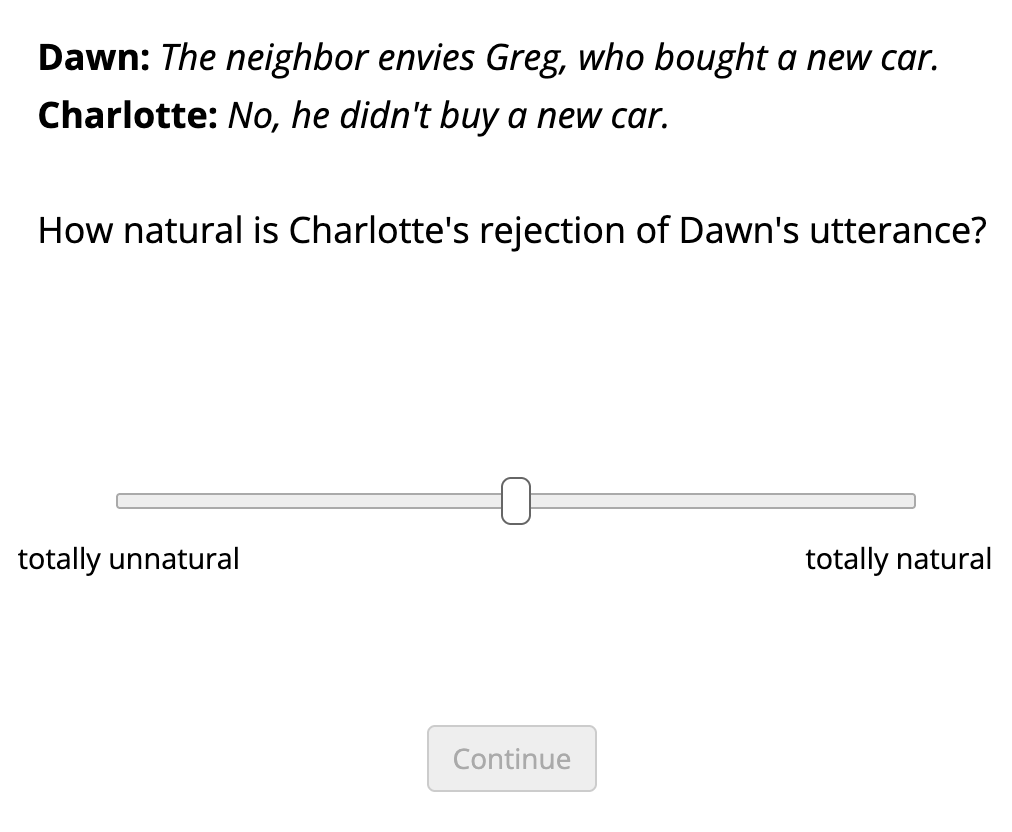
\includegraphics[width=0.47\textwidth]{figures/trialExp3}}%
    \label{fig:trialExp3}
  }
  \hfill
  \subfigure[Exp.~4: `yes, but' diagnostic]{%
    \fbox{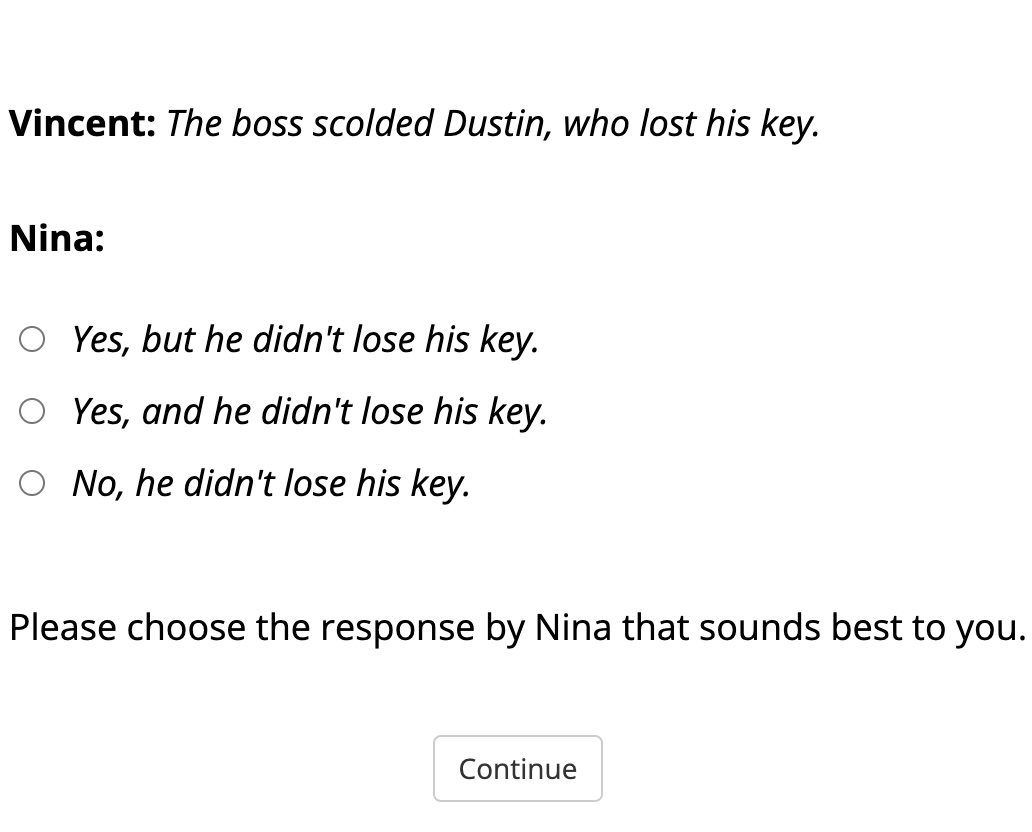
\includegraphics[width=0.47\textwidth]{figures/trialExp4}}%
    \label{fig:trialExp4}
  }

  \caption{Sample trials in (a) Exp.~1, (b) Exp.~2, (c) Exp.~3, and (d) Exp.~4.}
  \label{fig:trials}
  \end{figure}

  Each of the seven contents in \ref{stims} was instantiated by one of the seven items shown in \ref{items} in each of the four experiments.
 
  \ex.\label{items}
  \a. Jack saw the murder.
  \b. Raul cheated on his wife.
  \c. Ann stole the money.
  \d. Danny ate the last cupcake.
  \b. Lucy broke the plate.
  \b. Dustin lost his key.
  \b. Greg bought a new car.
  \z.

  Each experiment also included two control stimuli, which functioned as attention checks: one stimulus was expected to receive a response at one end of the slider (Exps.~1-3) or a `no' response (Exp.~4); the other control stimulus was expected tor receive a response at the other end of the slider (Exps.~1-3) or a `yes' response (Exp.~4). See Supplement \ref{supp:stims} for the control stimuli used in Exps.~1-4.

  In each of the four experiments, each participant's set of items was generated by randomly combining each of the seven contents in \ref{stims} with a unique content in \ref{items}. Participants completed a total of 9 trials, namely 7 target trials and the same 2 control trials. Trial order was randomized.

  After completing the experiment, participants filled out a short optional demographic survey. To encourage truthful responses, participants were told that they would be paid no matter what answers they gave in the survey. 

  \subsubsection{Data exclusion}

  We excluded the data of participants who did not self-identify as native speakers of
  American English and of participants whose responses to either one of the two control trials was more than 2 sd away from the group mean (Exps.~1-3) or whose responses to either one of the two control trials was wrong (Exp.~4).   Table \ref{t:excluded} shows how many participants were excluded in each experiment, the properties of the remaining participants, and the number of data points that entered into the analyses.

  \begin{table}[h!]
  \centering
  \begin{tabular}{l | r r | r r  | r }
               & \multicolumn{2}{c|}{\bf exclusion criterion} & \multicolumn{2}{c|}{\bf remaining participants} & data \\ 
              & language & fillers & ages (mean age) & f/m/nb/dnd &  points \\ \hline
  Exp.~1 (QUD   & 1 &  10 &  18-81 (41.1) & 36/32/0/1 & 621 \\ 
  Exp.~2 (asking whether) &  2 &  4 & 22-74 (38.7) & 45/27/1/1 & 666 \\ 
  Exp.~3  (direct dissent) &  2 &  7 & 18-77 (39.5) & 44/25/1/1  & 639 \\ 
  Exp.~4  (yes, but) & 4 & 4 & 19-67 (38.5)  & 43/27/2/0 & 648 \\ 
  \hline
  \end{tabular}
  \caption{Information from Exps.~1-4 about the number of participants whose data was excluded based on their self-declared language (variety) and the fillers, about the remaining participants, and about the number of data points that entered into the analysis.}\label{t:excluded}
  \end{table}

  \subsection{Results}
  
  Fig.~\ref{fig:results} plots the results of the four experiments by the expression that is associated with the seven target contents: panel (a) shows the mean naturalness ratings in Exp.~1 (QUD diagnostic), panel (b) the mean `asking whether' ratings in Exp.~2 (`asking whether' diagnostic), panel (c) the mean naturalness ratings in Exp.~3 (`direct dissent' diagnostic) and panel (d) the proportion of `no' choices in Exp.~4 (`yes, but' diagnostic).  We observe that the results of the four experiments differ in the range of the (mean or proportion of) ratings, that is, the difference between the largest and smallest ratings. {\bf JT: redo, now that plots different} The range is largest in Exp.~2 (`asking whether' diagnostic), at .74 (.01 to .83) and smallest in Exp.~3 (`direct dissent' diagnostic), at .13 (.64 to .78). The results of Exp.~1 (QUD diagnostic, with a range of .27 (.51 to .77) and Exp.~4 (`yes, but' diagnostic), with a range of .46 (.5 to .96), fall in-between. This result suggests that the four diagnostics that were implemented in Exps.~1-4 differ in how much they differentiate between the seven contents investigated, with the `asking whether' diagnostic showing the most differentiation and the `direct dissent' and the QUD diagnostic showing the least differentiation.

  \lh{some discussion of how this relates to the AI main clause controls could be useful and interesting; maybe mention here. (leaving out the \enquote{not-at-issue} controls, as they dont quite work as such)}

  We also observe that the results of the four experiments differ in the relative ratings that the seven contents received. The only two contents that received consistent relative ratings across all four experiments are the contents of the complement of \emph{discover} and \emph{confess}: The content of the complement of \emph{discover} received higher ratings (at least numerically) across all four experiments than that of \emph{confess}. There is no other pair of expressions for which that is the case. For instance, whereas the content of the complement of \emph{confirm} received (numerically) higher ratings than that of \emph{know} in Exps.~1 and 2, the opposite pattern is observed in Exps.~3 and 4. This difference between the results of the experiments is quantified in the Spearman rank correlations  {\bf JT: redo} in Table \ref{t:spearman}.\footnote{The Spearman rank correlation coefficient, a value between -1 and 1, is a nonparametric measure of rank correlation: the higher the coefficient, the more the relation between the the two variables can be described using a monotonic function. If the coefficient is positive, the value of one variable tends to increase with an increase in the other. In the case of our experiments, a coefficient of 1 for two experiments would mean that there is a perfectly monotone increasing relation between the mean ratings of the seven contents in the two experiments: for any two contents c1 and c2, if c1 ranks below c2 in one experiment (that is, the mean rating of c1 is lower than that of c2), then that ranking is preserved in the other experiment.} The rank correlations are particularly low for for Exp.~1 compared to the other three experiments, which is due at least in part to the fact that the content of the complement of \emph{be right} is the most not-at-issue content of the seven contents in Exp.~1, but among the least not-at-issue in the other three experiments. These results suggests that the four diagnostics as implemented in Exps.~1-4 interact differently with the seven contents investigated.

  \lh{should the spearman-rank correlation values be reported with a p-value and sample size as well?}

  \lh{Here, we should discuss that \emph{be right that p} gets low acceptability ratings with the QUD test because of reasons independent to the (not-)at-issueness of the tested content, namely the factor that another not-at-issue inference (that someone said p) is presupposed, and therefore the utterance is less acceptable following a question that doesnt also presuppose that someone said p. This complication is also an example of an interacting factors that, I think, is obscured by reversing the scale and therefore removing the representation from our intuitive understanding of the acceptability rating task.}

  \lh{include here: calculation of rank correlation without \emph{be right}. Does that improve correlations with QUD task, how much?}

  \begin{table}[ht!]
    \centering
    \begin{tabular}{l | c c c c}
    & Exp.~1 & Exp.~2 & Exp.~3 & Exp.~4 \\ \hline
    Exp.~1 (QUD diagnostic) & \cellcolor{lightgray} & .11 & -.29 & -.18 \\
    Exp.~2 (`asking whether' diagnostic) & \cellcolor{lightgray} & \cellcolor{lightgray} & .64 &.79 \\
    Exp.~3 (`direct dissent' diagnostic) & \cellcolor{lightgray}& \cellcolor{lightgray} & \cellcolor{lightgray} & .79  \\
    \hline
    % Exp.~4 (`yes, but' diagnostic) & & & & \cellcolor{lightgray} \\ \hline
    \end{tabular}
  \caption{Spearman rank correlations between the results of Exps.~1-4.}\label{t:spearman}
  \end{table}
  
 
  \begin{figure}[h!]
    \centering
    % Top row
    \subfigure[Exp.~1 (QUD diagnostic)]{%
      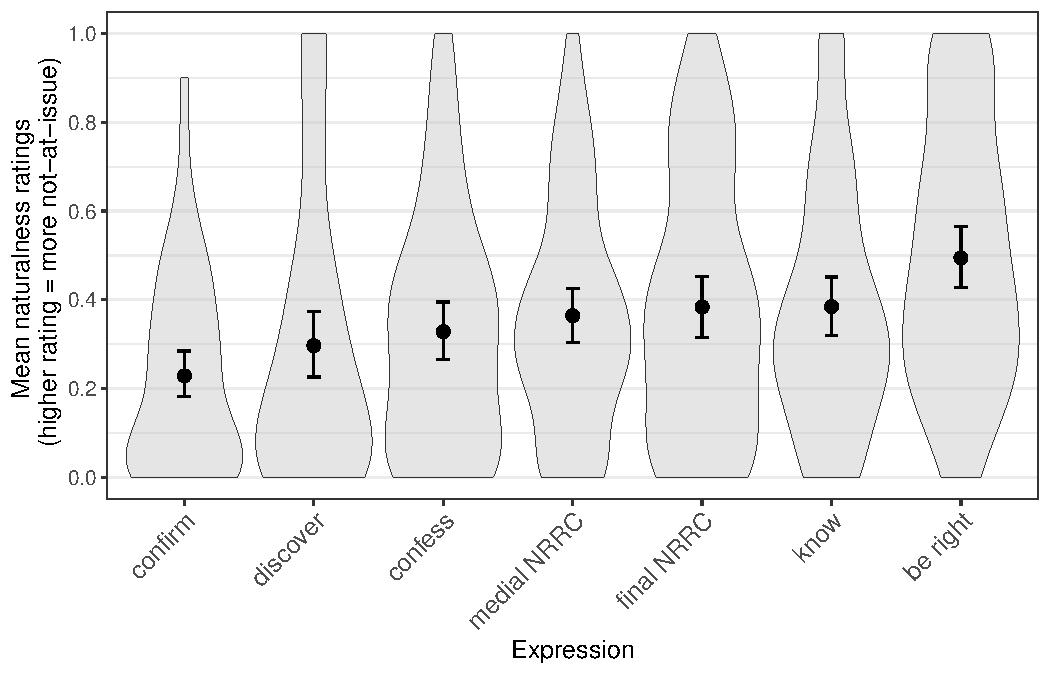
\includegraphics[width=0.48\linewidth]{../../results/exp1/graphs/mean-ratings.pdf}%
      \label{fig:qud}
    }
    \hfill
    \subfigure[Exp.~2 (`asking whether' diagnostic)]{%
      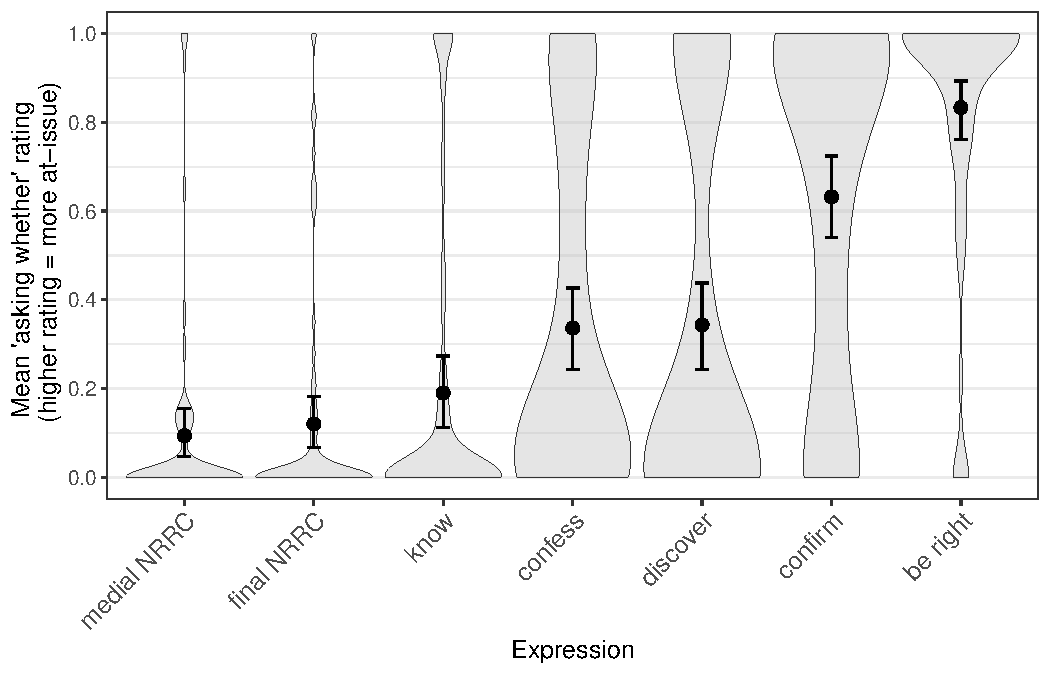
\includegraphics[width=0.48\linewidth]{../../results/exp2/graphs/mean-ratings.pdf}%
      \label{fig:AK}
    }

    % \vspace{1em}

    % Bottom row
    \subfigure[Exp.~3 (`direct dissent' diagnostic)]{%
      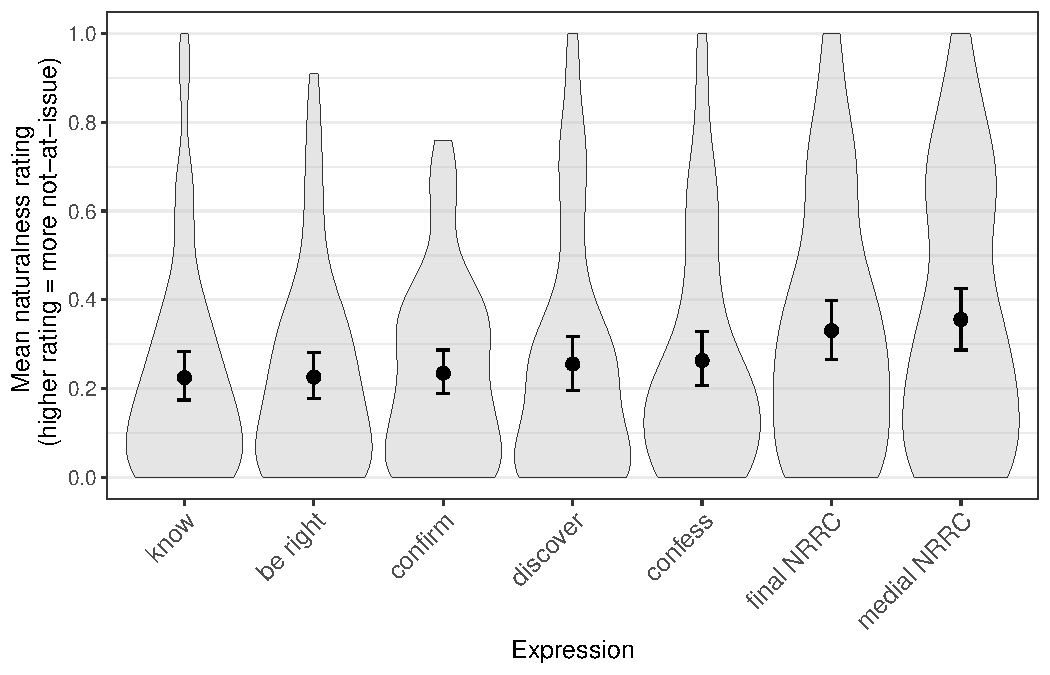
\includegraphics[width=0.48\textwidth]{../../results/exp3/graphs/mean-ratings.pdf}%
      \label{fig:dd}
    }
    \hfill
    \subfigure[Exp.~4 (`yes, but' diagnostic)]{%
      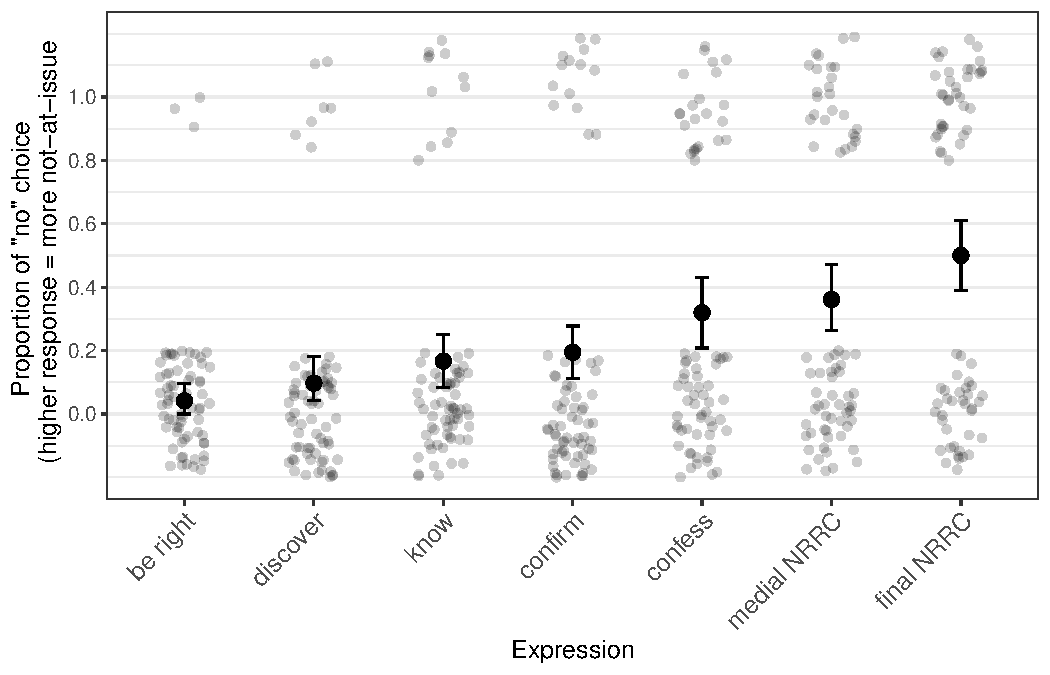
\includegraphics[width=0.48\textwidth]{../../results/exp4/graphs/mean-ratings.pdf}%
      \label{fig:yb}
    }
  \caption{Results of Exps.~1--4.
    Panels (a)--(c) show the mean responses by expression for (a) Exp.~1 (QUD diagnostic),  (b) Exp.~2 (`asking whether' diagnostic), and (c) Exp.~3 (`direct dissent' diagnostic); panel (d) shows the proportion of `no' choices by expression in Exp.~4 (`yes, but' diagnostic). Error bars indicate 95\% bootstrapped confidence intervals. Violin plots in panels (a)-(c) show the kernel probability density of individual participants' ratings. Gray dots in panel (d) represent individual participant responses (`no' vs.\ `yes', jittered vertically and horizontally for legibility).}
  \label{fig:results}
  \end{figure}

  Finally, the results of the experiments differ with respect to whether distinctions between contents from prior literature are observed. Fig.~\ref{fig:pairwise} presents the results of posthoc pairwise comparisons of the estimated means/proportions for each content using the `emmeans' package (\citealt{emmeans}) in R (\citealt{r}). The input to the pairwise comparisons were mixed-effects beta regression models (Exps.~1-3) or a mixed-effects logistic regression model (Exp.~4) with weakly informative priors that were fit using the `brms' package (\citealt{buerkner2017}). The models predicted the  ratings\footnote{To model the ratings in Exps.~1-3 using a beta regression, the ratings were first transformed from the interval [0,1] to the interval (0,1) using the method proposed in \citealt{smithson-verkuilen2006}.} from a fixed effect of expression (with treatment coding and `be right' as reference level) and included random by-participant and by-item intercepts. The output of the pairwise comparison were 95\% highest density intervals (HDIs) of estimated marginal mean differences between each of the expressions. We assume that two contents differ if their HDI does not include 0.\footnote{The full model outputs are available in the folder {\bf where?} in the repository linked in footnote \ref{f:github}.}

  \lh{I think that \emph{be right} would be a good choice for a reference level, if we only have exps 2--4, because in all of those, that seems to be the condition with the least amount of variation. In exp. 1, however, this condition has much more variation. I think that the pairwise comparison of marginal posteriors between the conditions will always also quantify over the uncertainty in the baseline condition, so this could be part of reason for why we see fewer significant differences in exp. 1 than others.}

  Recall that \citealt{syrett_experimental_2015}, using a variant of the direct-dissent diagnostic, found that sentence-medial NRRCs are more not-at-issue than sentence-final ones. As shown in Figs.~\ref{fig:results} and \ref{fig:pairwise}, no difference is observed in Exps.~1-3; in Exp.~4 (`yes, but' diagnostic), sentence-final NRRCs are more not-at-issue than sentence-medial ones.  This result suggests that none of the diagnostics as implemented in Exps.~1-4 predict that sentence-medial NRRCs are more not-at-issue than sentence-final ones, contrary to \citeposs{syrett_experimental_2015} result.

  \lh{some more discssion here would be interesting (bullets below)}

  \begin{itemize}
    \item include some discussion of task differences
    \item also compare to yes but test, where we actually see the reverse difference than would be expected from S+K
    \item WHY? response task may make a difference, but is there anything about the contents that is different?\bigskip
  \end{itemize}
  
  Recall also that \citealt{tonhauser_how_2018} and \citealt{degen-tonhauser-glossa}, using the `asking whether' diagnostic, observed that the content of the clausal complement of \emph{know} was more not-at-issue than that of \emph{discover}, which in turn was more not-at-issue than that of \emph{confess}, which in turn was more not-at-issue than that of \emph{confirm}, which in turn was more not-at-issue than that of \emph{be right}.  As shown in Figs.~\ref{fig:results} and \ref{fig:pairwise}, these differences are replicated in Exp.~2 (`asking whether' diagnostic), except for the contents of the complement of \emph{confess} and \emph{discover}. In Exp.~1 (QUD diagnostic), the content of the complement of \emph{confirm} is less not-at-issue than that of \emph{confess} and \emph{know}, but the only other difference that is observed is that the content of the complement of \emph{be right} is less at-issue than those of the other predicates -- the direction of this difference is the opposite from that observed in prior literature and the other experiments. In Exp.~3..., Finally, in Exp.~4, the content of the complement of \emph{be right} is more at-issue than those of \emph{confirm, confess} and \emph{know}, that of \emph{confirm} is more at-issue than that of \emph{confess}, and that of \emph{discover} is more at-issue than that of \emph{confess}. These results suggest that the diagnostics, as implemented in Exps.~1-4, differ in whether they predict differences in at-issueness between the contents of the complements of the five clause-embedding predicates included in the experiments.

  %Exp 1
  %min: 0.5055072
  %max: 0.7713043
  %range: 0.2657971

  %Exp 2
  %min: 0.09364865
  %max: 0.8332432
  %range: 0.7395946

  %Exp 3
  %min: 0.6443662
  %max: 0.7752113
  %range: 0.1308451

  %Exp 4
  %min: .5
  %max: 0.958
  %range: 0.458

  \addtolength{\tabcolsep}{-.19em}

  \begin{figure}[!h]
    \centering
    \subfigure[Exp.~1 (QUD diagnostic)]{%
    \begin{tabular}{r | ccccccc}
    & \rots{be right} & \rots{confirm} & \rots{discover} & \rots{confess} & \rots{know} & \rots{final NRRC} & \rots{medial NRRC} \\
    \hline
     be right & \cellcolor{black} & \cellcolor{red} & \cellcolor{red} & \cellcolor{red} & \cellcolor{red} & \cellcolor{red} & \cellcolor{red} \\ 
  confirm & \cellcolor{black} & \cellcolor{black} & \cellcolor{white} & \cellcolor{blue} & \cellcolor{blue} & \cellcolor{blue} & \cellcolor{blue} \\ 
  discover & \cellcolor{black} & \cellcolor{black} & \cellcolor{black} & \cellcolor{white} & \cellcolor{white} & \cellcolor{blue} & \cellcolor{blue} \\ 
  confess & \cellcolor{black} & \cellcolor{black} & \cellcolor{black} & \cellcolor{black} & \cellcolor{white} & \cellcolor{white} & \cellcolor{white} \\ 
  know & \cellcolor{black} & \cellcolor{black} & \cellcolor{black} & \cellcolor{black} & \cellcolor{black} & \cellcolor{white} & \cellcolor{white} \\ 
  final NRRC & \cellcolor{black} & \cellcolor{black} & \cellcolor{black} & \cellcolor{black} & \cellcolor{black} & \cellcolor{black} & \cellcolor{white} \\ 
  medial NRRC & \cellcolor{black} & \cellcolor{black} & \cellcolor{black} & \cellcolor{black} & \cellcolor{black} & \cellcolor{black} & \cellcolor{black} \\ 
  

    \hline
    \end{tabular}}
    \hfill
    \subfigure[Exp.~2 (`asking whether' diagnostic)]{%
    \begin{tabular}{r | ccccccc}
    & \rots{be right} & \rots{confirm} & \rots{discover} & \rots{confess} & \rots{know} & \rots{final NRRC} & \rots{medial NRRC} \\
    \hline
     be right & \cellcolor{black} & \cellcolor{blue} & \cellcolor{blue} & \cellcolor{blue} & \cellcolor{blue} & \cellcolor{blue} & \cellcolor{blue} \\ 
  confirm & \cellcolor{black} & \cellcolor{black} & \cellcolor{blue} & \cellcolor{blue} & \cellcolor{blue} & \cellcolor{blue} & \cellcolor{blue} \\ 
  discover & \cellcolor{black} & \cellcolor{black} & \cellcolor{black} & \cellcolor{white} & \cellcolor{blue} & \cellcolor{blue} & \cellcolor{blue} \\ 
  confess & \cellcolor{black} & \cellcolor{black} & \cellcolor{black} & \cellcolor{black} & \cellcolor{blue} & \cellcolor{blue} & \cellcolor{blue} \\ 
  know & \cellcolor{black} & \cellcolor{black} & \cellcolor{black} & \cellcolor{black} & \cellcolor{black} & \cellcolor{blue} & \cellcolor{blue} \\ 
  final NRRC & \cellcolor{black} & \cellcolor{black} & \cellcolor{black} & \cellcolor{black} & \cellcolor{black} & \cellcolor{black} & \cellcolor{white} \\ 
  medial NRRC & \cellcolor{black} & \cellcolor{black} & \cellcolor{black} & \cellcolor{black} & \cellcolor{black} & \cellcolor{black} & \cellcolor{black} \\ 
  

    \hline
    \end{tabular}}

    \subfigure[Exp.~3 (`direct dissent' diagnostic)]{%
    \begin{tabular}{r | ccccccc}
    & \rots{be right} & \rots{confirm} & \rots{discover} & \rots{confess} & \rots{know} & \rots{final NRRC} & \rots{medial NRRC} \\
    \hline
     be right & \cellcolor{black} & \cellcolor{white} & \cellcolor{white} & \cellcolor{white} & \cellcolor{white} & \cellcolor{blue} & \cellcolor{blue} \\ 
  confirm & \cellcolor{black} & \cellcolor{black} & \cellcolor{white} & \cellcolor{white} & \cellcolor{white} & \cellcolor{blue} & \cellcolor{blue} \\ 
  discover & \cellcolor{black} & \cellcolor{black} & \cellcolor{black} & \cellcolor{white} & \cellcolor{white} & \cellcolor{blue} & \cellcolor{blue} \\ 
  confess & \cellcolor{black} & \cellcolor{black} & \cellcolor{black} & \cellcolor{black} & \cellcolor{white} & \cellcolor{white} & \cellcolor{blue} \\ 
  know & \cellcolor{black} & \cellcolor{black} & \cellcolor{black} & \cellcolor{black} & \cellcolor{black} & \cellcolor{blue} & \cellcolor{blue} \\ 
  final NRRC & \cellcolor{black} & \cellcolor{black} & \cellcolor{black} & \cellcolor{black} & \cellcolor{black} & \cellcolor{black} & \cellcolor{white} \\ 
  

    \hline
    \end{tabular}}
    \hfill
    \subfigure[Exp.~4 (`yes, but' diagnostic)]{%
    \begin{tabular}{r | ccccccc}
    & \rots{be right} & \rots{confirm} & \rots{discover} & \rots{confess} & \rots{know} & \rots{final NRRC} & \rots{medial NRRC} \\
    \hline
     be right & \cellcolor{black} & \cellcolor{blue} & \cellcolor{white} & \cellcolor{blue} & \cellcolor{blue} & \cellcolor{blue} & \cellcolor{blue} \\ 
  confirm & \cellcolor{black} & \cellcolor{black} & \cellcolor{white} & \cellcolor{blue} & \cellcolor{white} & \cellcolor{blue} & \cellcolor{blue} \\ 
  discover & \cellcolor{black} & \cellcolor{black} & \cellcolor{black} & \cellcolor{blue} & \cellcolor{white} & \cellcolor{blue} & \cellcolor{blue} \\ 
  confess & \cellcolor{black} & \cellcolor{black} & \cellcolor{black} & \cellcolor{black} & \cellcolor{red} & \cellcolor{blue} & \cellcolor{white} \\ 
  know & \cellcolor{black} & \cellcolor{black} & \cellcolor{black} & \cellcolor{black} & \cellcolor{black} & \cellcolor{blue} & \cellcolor{blue} \\ 
  final NRRC & \cellcolor{black} & \cellcolor{black} & \cellcolor{black} & \cellcolor{black} & \cellcolor{black} & \cellcolor{black} & \cellcolor{red} \\ 
  medial NRRC & \cellcolor{black} & \cellcolor{black} & \cellcolor{black} & \cellcolor{black} & \cellcolor{black} & \cellcolor{black} & \cellcolor{black} \\ 
  

    \hline
    \end{tabular}}

  \caption{Pairwise differences between expressions,
    ordered from top to bottom and left to right by increasing mean in Exp.~2 (`asking whether' diagnostic). A white cell means that the 95\% HDI of the pair of the row expression and the column expression includes 0, a red cell means that the 95\% HDI does not include 0 and that the coefficient is positive (the row expression received a higher rating than the column expression), and a blue cell means that the 95\% HDI does not include 0 and the coefficient is negative (the row expression received a lower rating than the column expression).}
  \label{fig:pairwise}
  \end{figure}

  \newpage

  bla

  \newpage

  \subsection{Discussion}

  Exps.~1-4 were designed to compared the results of four different diagnostics of at-issueness that have been used in prior literature. The results of the experiments suggest that the diagnostics, in the particular way in which they were implemented in the experiments, differ on several dimensions. First, they differ in the extent to which they differentiate between the seven contents investigated, with the `asking whether' diagnostic of Exp.~2 showing the most differentiation and the `direct dissent' diagnostic of Exp.~3 showing the least. Second, the diagnostics as implemented differ in the way in which they interact with the seven contents. In particular, while the results of none of the experiments differentiated between sentence-medial and -final NRRCs, the results of Exp.~2 (`asking whether' diagnostic) distinguished between most of the contents of the complements of the five clause-embedding predicates, whereas the results of Exp.~xx (`' diagnostic) distinguished between the least of these contents.
  %
  \lh{Right, although the second is a measure of the first point. Revise: \enquote{diagnostics differ in the extent to which they differentiate between contents}, first this can be quantified by the range of means, second, by which differences between means there are}

  One of the most striking differences between the results of the experiments concerns the content of the complement of \emph{be right} in Exp.~1 (QUD diagnostic) vs.\ the other three experiments. As shown in panel (a) of Fig.~\ref{fig:results}, participants gave relatively high naturalness ratings to responses like that in \ref{beright.a}, suggesting that they did not take the response to fit the question. As discussed above, the content of the complement of \emph{be right} emerged as the most not-at-issue in Exp.~1. 

  \ex.
    \a.\label{beright.a}  Exp.~1 (QUD diagnostic) with \emph{be right}
    \\ {\bf Nora:} \emph{What did Lucy break?}
    \\ {\bf Leo:} \emph{Danny is right that she broke the plate.}
    \b.\label{beright.b} Exp.~2 (`asking whether' diagnostic )
    \\ {\bf Nora:} \emph{Is Danny right that she broke the plate?}
    \c.\label{beright.c} Exp.~3 (`direct dissent' diagnostic)
    \\ {\bf Nora:} \emph{Danny is right that she broke the plate.}
    \\ {\bf Leo:} \emph{No, she didn't break the plate.}
    \d.\label{beright.d} Exp.~4 (`yes, but' diagnostic)
    \\ {\bf Nora:} \emph{Danny is right that she broke the plate.}
    \\ {\bf Leo:} \emph{Yes, but she didn't break the plate.}
    \\ \hspace*{1cm} \emph{Yes, and she didn't break the plate.}
    \\ \hspace*{1cm} \emph{No, she didn't break the plate.}

  Why might this be? We hypothesize that this is because \emph{be right} signals that the question of whether Lucy broke the place must be salient in discourse. But no such discourse context is given and it is difficult to accommodate, so low naturalness ratings. This doesn't happen in the other diagnostics, shown in \ref{beright.b} to \ref{beright.d}.\footnote{When \emph{be right} is excluded, the Spearman rank correlations are:
    
   \begin{tabular}{l | c c c c}
   & Exp.~1 & Exp.~2 & Exp.~3 & Exp.~4 \\ \hline
   Exp.~1 (QUD diagnostic) & \cellcolor{lightgray} & .77 & .09 & .31 \\
   Exp.~2 (`asking whether' diagnostic) & \cellcolor{lightgray} & \cellcolor{lightgray} & .66 & .66 \\
   Exp.~3 (`direct dissent' diagnostic) & \cellcolor{lightgray}& \cellcolor{lightgray} & \cellcolor{lightgray} & .77  \\
   \hline
  % Exp.~4 (`yes, but' diagnostic) & & & & \cellcolor{lightgray} \\ \hline
   \end{tabular}} So, when using a particular diagnostic, one also has to worry about whether the expression might presuppose a particular context, if one wants to ask about how well an utterance fits the context.

   \begin{itemize}
     \item \lh{we can take more away from this observation. The correlations without our confounding condition should not be hidden away in a footnote. I even think that it should be included in the results section, before the discussion; (see my comments there, and in discussion section notes for suggestions on how to interpret this result).}

     \item \lh{Correlation between Exp. 1 and Exp. 2 is .77, suggesting that higher QUD-match ratings were strongly associated with higher asking-whether ratings.}

     \item \lh{Correlation between Exp. 3 and Exp. 4 is .77, suggesting that higher accptability ratings in the direct-dissent task were strongly associated with higher proportions of `yes'-answers.}

     \item \lh{However, the correlation between Exp. 1 and Exps. 3/4, respectively, is only weak to moderate, while the corratlation between Exp. 2 and Exps. 3/4, respectively, would be characterized as strong, but again, is lower than when comparing the question-based and assertion-based diagnostics to each other. Is there any way to quantify this, or do significance testing on that?}

     \item \lh{The correlation between all diagnostics suggests that there is an underlying property that they all are sensitive to, but the fact that the correlation is higher between those diagnostics that share theoretical assumptions about at-issueness should tell us something too. (what exactly? this is hard to say on an appropriate level of abstraction; I think concluding that they are sensitive to different underlying phenomena would be too strong here)}

   \end{itemize}
   
  As mentioned above, none of our experiments replicated the effect reported in \citealt{syrett_experimental_2015}, that sentence-final NRRCs are more at-issue than sentence-medial ones. This includes Exp.~3, which implemented a variant of the `direct dissent' diagnostic that was used in \citealt{syrett_experimental_2015}. A difference between our Exp.~3 and Exp.~2 in \citealt{syrett_experimental_2015}, aside from the stimuli, is that we asked for naturalness ratings and they implemented it as a forced choice: do you choose to dissent with the main clause content or the content of the NRRC. An interesting follow-up would be to see whether our stimuli with the forced choice can reproduce their result.

  \lh{even more: Exp. 4, our forced-choice assent/dissent-based task shows the opposite effect.}

  One of the most noticable differences between the results of the experiments is that Exp.~2 has much larger range and differentiation among the contents. Why might this be? It is the only diagnostic where the expression/content occurs in a polar question. We hypothesize that the polar question embedding highlights at-issueness differences. Content is differently suitable to partition the context set, with some content really well able to do this and other content not, and other content inbetween. All the other diagnostics rely on anaphoric accessibility of the proposition or how well it can address a question in prior discourse.

  \lh{nice! Also, previous literature has suggested a difference in theoretical assumptions based on whether the status of a content as (not-)at-issue is introduced as a QUD or as the proposal contributed by an assertion. however, the QUD-test still tests the at-issueness of content in an assertive utterance relative to a preceding question. no previous literature has suggested that the speech act of the content being tested itself plays a large role.
  }
     
  To investigate whether it is really embedding polar question that creates this differentiation, it would be good to investigate a diagnostic that also embeds the expression/content in a polar question but uses a different assumption about at-issueness. This is what we do in the next section.
        
\section{Experiments 5-6 \label{sec:3_more-experiments}}

  Exps.~5 and 6 allow us to investigate the question of whether the great differentiation observed in Exp.~2 (`asking whether' diagnostic) is due to the fact that the contents were embedded in a polar interrogative or due to the response task. The design of Exp.~5 is like that of Exp.~2 except that it measures at-issueness for the contents of the complements of the 20 clause-embedding predicates of \citealt{tonhauser_how_2018} and \citealt{degen-tonhauser-glossa}. Exp.~6 also investigates these contents, but uses a version of the  `direct assent' diagnostic where the contents are embedded in a polar interrogative. As shown in \ref{exp6}, the expression/content occurs in a polar question and the response directly assents with the content. 

    \ex.
    \a.\label{exp5} Exp.~5 (`asking whether' diagnostic )
    \\ {\bf Nora:} \emph{Is xx right that Lucy broke the plate?}
    \\ Question to participants: Is Nora asking whether Lucy broke the plate?
    \b.\label{exp6} Exp.~6 (`direct dissent' diagnostic)
    \\ {\bf Nora:} \emph{Is XX right that Lucy broke the plate?}
    \\ {\bf Leo:} \emph{Yes, she didn't break the plate.}
    \\ Question to participants: How natural is Leo's response to Nora's question?
    
  Both experiments measured not just at-issueness but also projection. The projection data were reported in \citealt{hofmann-etal2024}); here we focus on the at-issueness data, which have not yet been reported.

    \subsection{Methods}
    
    \subsubsection{Participants}

      We recruited 300 participants on Amazon's Mechanical Turk platform for Exp.~5 and 250 participants on Prolific for Exp.~6.\footnote{Exp.~5 was run in August 2019 and Exp.~6 in August 2021.} Participants recruited on Amazon's Mechanical Turk platform had U.S.\ IP addresses and at least 99\% of previous HITs approved. Participants recruited on Prolific had registered on the platform as living in the USA, to be born in the USA and as having English as their first language. They had an approval rate of at least 99\%.  Table \ref{t:recruited2} shows the age and gender distributions of the recruited participants.

      \begin{table}[h!]
      \centering
      \begin{tabular}{l | c | r r r }
                  & recruited & ages (mean age) & f/m/nb/dnd \\ \hline
      Exp.~5 (asking whether) & 300 & 19-74 (38.2) & --/--/--/--  \\
      Exp.~6 (direct assent) & 250 & 18-58 (25.5)  & 201/43/6/0  \\
      \hline
      \end{tabular}

      \caption{Information about the participants recruited in Exps.~5-6 (f = female, m = male, nb = nonbinary, dnd = did not disclose; gender information was not collected in Exp.~5).}\label{t:recruited2}
      \end{table}

    \subsubsection{Materials and procedure}
    
    The target stimuli in both Exps.~4-5 were 400 polar interrogatives that consisted of one of the 20 clause-embedding predicates in \ref{ex:predicates} and one of 20 embedded clauses (provided in Supplement A). 
    
    
    The at-issueness and projection blocks also included 6 control trials each, which functioned as attention checks: The contents of these items were expected to be at-issue and not to project. The same 6 contents were also used to form 6 filler trials in the prior block. These filler items were not used to assess participants' attention. For the full set of control and filler items see Supplement \ref{a-stim}.

              Each participant saw a random set of 26 stimuli: Each set contained one target stimulus for each of the 20 clause-embedding predicates (each with a unique complement clause) and the same six control stimuli.\footnote{Each participant saw their set of 26 stimuli twice, once in the projection block and once in the at-issueness block. Block order was randomized. As mentioned above, we focus here on the projection ratings.} Trial order was randomized.
  	
              Participants were asked to imagine that they are at a party and that, when walking into the kitchen, they overhear somebody say something to somebody else.
              
              On each trial, they read an utterance and gave a response to the `certain that' question on a slider marked `no' (coded as 0) at one end and `yes' (coded as 1) at the other. A sample trial %from Exps.~1
              is shown in Figure~\ref{fig:trial}.            
              Following \citealt{tonhauser_how_2018}, higher ratings of speaker certainty could reflect one of two things. First, higher certainty ratings could reflect greater speaker commitment towards the CC, and therefore greater projection. This assumes that speaker commitment is interpreted in a gradient way. Second, higher certainty ratings could reflect a higher probability that an interpreter takes the speaker to be committed to the CC.  On this interpretation, speaker commitment may be a binary, categorical property and projection variation is a result of uncertainty about speaker commitment. In this paper, we remain agnostic about the underlying interpretation of projectivity as a gradient property (for discussion, see  \citealt{grove_factivity_2023}).
              
   After completing the experiment, participants filled out a short optional demographic survey. To encourage truthful responses, participants were told that they would be paid no matter what answers they gave in the survey.

    \subsubsection{Data exclusion}
    
  We excluded the data of participants who did not self-identify as native speakers of American
  English, of participants whose responses to the projection or at-issueness controls were more than 2 sd away from the group mean, and of participants who always selected roughly the same point on the response scale for the target stimuli. To identify such participants, we first identified participants whose mean variance on the target stimuli was more than 2 sd below the group mean variance and then manually inspecting their response patterns. Due to a programming error, 5 participants took Exp.~5 more than once. Since we were not able to identify which submission was their first submission, the data of these participants was also excluded. Table \ref{t:excluded2} shows how many participants were excluded in each experiment, the properties of the remaining participants, and the number of data points that entered into the analyses.

  {\bf table should show final number of participants, exp 5: 242; exp 6: }
    
  \begin{table}[h!]
    \centering
    \begin{tabular}{l | r r r | r r  | r }
                 & \multicolumn{3}{c|}{\bf exclusion criterion} & \multicolumn{2}{c|}{\bf remaining participants} & data \\ 
                & language & controls & variance & ages (mean age) & f/m/nb/dnd &  points \\ \hline
    Exp.~5 (asking whether)  & 7 &  35 & 0 &  21-74 (39.2) & --/--/--/-- & 6292 \\ 
    Exp.~6 (direct assent) &  5 &  24 & 1 & 18-58 (24.9) & 187/28/5/0 & 5720 \\ 
    \hline
    \end{tabular}
    \caption{Information from Exps.~5-6 about the number of participants whose data was excluded based on their self-declared language and language variety (`language'), the controls, and the variance of their responses, about the remaining participants, and about the number of at-issueness data points that entered into the analysis.}\label{t:excluded2}
    \end{table}

    \subsection{Results}
    
    Spearman rank = .93

    \begin{figure}[h!]
      \centering
      
      \subfigure[Exp.~5 (`asking whether' diagnostic)]{%
        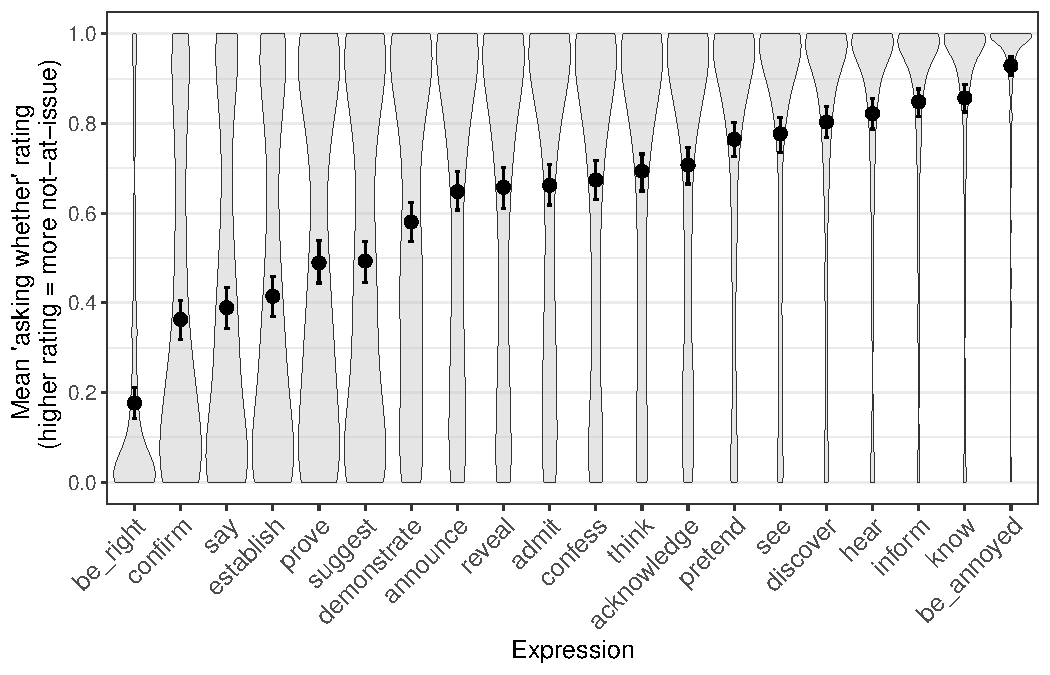
\includegraphics[width=0.7\linewidth]{../../results/exp5/graphs/mean-ratings.pdf}%
        \label{fig}
      }

      \subfigure[Exp.~6 (`direct assent' diagnostic)]{%
        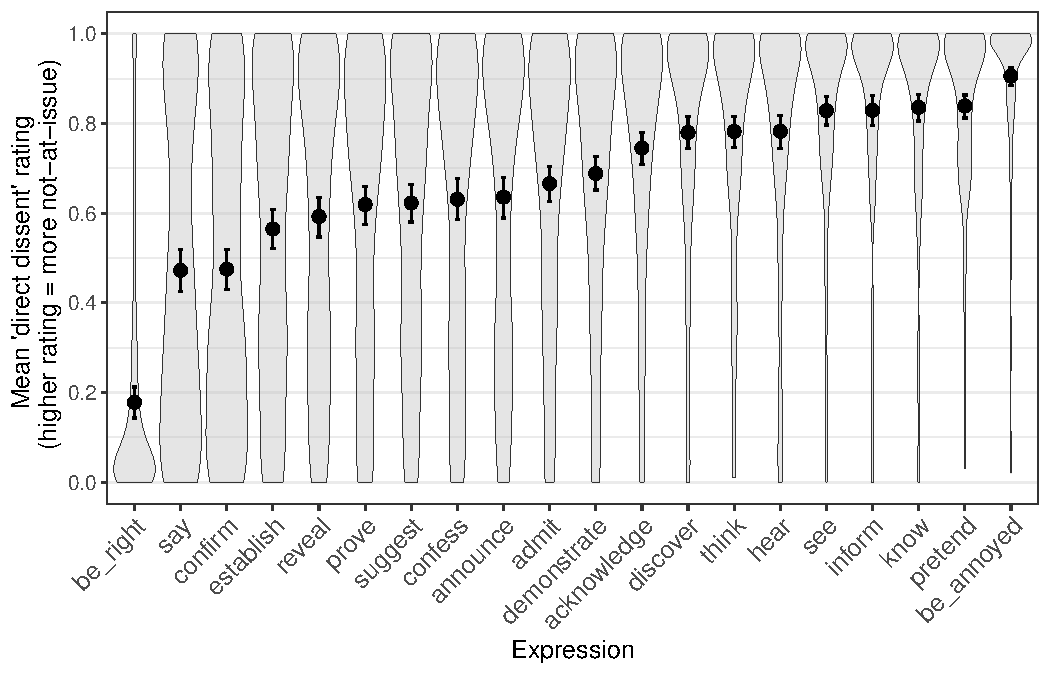
\includegraphics[width=0.7\linewidth]{../../results/exp6/graphs/mean-ratings.pdf}%
        \label{fig}
      }

      \caption{Results of Exps.~5-6. The panels show the mean ratings by expression for (a) Exp.~5 (asking whether diagnostic) and (b) Exp.~2 (direct assent diagnostic). Error bars indicate 95\% bootstrapped confidence intervals. Violin plots show the kernel probability density of individual participants' ratings.}
      \label{fig:results2}
    \end{figure}
    
  % \addtolength{\tabcolsep}{-.19em}

    \begin{figure}[!h]
    \centering

    \subfigure[Exp.~5 (`asking whether' diagnostic)]{%
    \begin{tabular}{r | ccccc ccccc ccccc ccccc}
    & \rots{be right} & \rots{confirm} & \rots{say} & \rots{establish} & \rots{prove} & \rots{suggest} & \rots{demonstrate} & \rots{announce} & \rots{reveal} & \rots{admit} & \rots{confess} & \rots{think} & \rots{acknowledge} & \rots{pretend} & \rots{see} & \rots{discover} & \rots{hear} & \rots{inform} & \rots{know} & \rots{be annoyed} \\
   \hline
     be right & \cellcolor{black} & \cellcolor{blue} & \cellcolor{blue} & \cellcolor{blue} & \cellcolor{blue} & \cellcolor{blue} & \cellcolor{blue} & \cellcolor{blue} & \cellcolor{blue} & \cellcolor{blue} & \cellcolor{blue} & \cellcolor{blue} & \cellcolor{blue} & \cellcolor{blue} & \cellcolor{blue} & \cellcolor{blue} & \cellcolor{blue} & \cellcolor{blue} & \cellcolor{blue} & \cellcolor{blue} \\ 
  confirm & \cellcolor{black} & \cellcolor{black} & \cellcolor{white} & \cellcolor{white} & \cellcolor{blue} & \cellcolor{blue} & \cellcolor{blue} & \cellcolor{blue} & \cellcolor{blue} & \cellcolor{blue} & \cellcolor{blue} & \cellcolor{blue} & \cellcolor{blue} & \cellcolor{blue} & \cellcolor{blue} & \cellcolor{blue} & \cellcolor{blue} & \cellcolor{blue} & \cellcolor{blue} & \cellcolor{blue} \\ 
  say & \cellcolor{black} & \cellcolor{black} & \cellcolor{black} & \cellcolor{white} & \cellcolor{blue} & \cellcolor{blue} & \cellcolor{blue} & \cellcolor{blue} & \cellcolor{blue} & \cellcolor{blue} & \cellcolor{blue} & \cellcolor{blue} & \cellcolor{blue} & \cellcolor{blue} & \cellcolor{blue} & \cellcolor{blue} & \cellcolor{blue} & \cellcolor{blue} & \cellcolor{blue} & \cellcolor{blue} \\ 
  establish & \cellcolor{black} & \cellcolor{black} & \cellcolor{black} & \cellcolor{black} & \cellcolor{blue} & \cellcolor{blue} & \cellcolor{blue} & \cellcolor{blue} & \cellcolor{blue} & \cellcolor{blue} & \cellcolor{blue} & \cellcolor{blue} & \cellcolor{blue} & \cellcolor{blue} & \cellcolor{blue} & \cellcolor{blue} & \cellcolor{blue} & \cellcolor{blue} & \cellcolor{blue} & \cellcolor{blue} \\ 
  prove & \cellcolor{black} & \cellcolor{black} & \cellcolor{black} & \cellcolor{black} & \cellcolor{black} & \cellcolor{white} & \cellcolor{blue} & \cellcolor{blue} & \cellcolor{blue} & \cellcolor{blue} & \cellcolor{blue} & \cellcolor{blue} & \cellcolor{blue} & \cellcolor{blue} & \cellcolor{blue} & \cellcolor{blue} & \cellcolor{blue} & \cellcolor{blue} & \cellcolor{blue} & \cellcolor{blue} \\ 
  suggest & \cellcolor{black} & \cellcolor{black} & \cellcolor{black} & \cellcolor{black} & \cellcolor{black} & \cellcolor{black} & \cellcolor{blue} & \cellcolor{blue} & \cellcolor{blue} & \cellcolor{blue} & \cellcolor{blue} & \cellcolor{blue} & \cellcolor{blue} & \cellcolor{blue} & \cellcolor{blue} & \cellcolor{blue} & \cellcolor{blue} & \cellcolor{blue} & \cellcolor{blue} & \cellcolor{blue} \\ 
  demonstrate & \cellcolor{black} & \cellcolor{black} & \cellcolor{black} & \cellcolor{black} & \cellcolor{black} & \cellcolor{black} & \cellcolor{black} & \cellcolor{blue} & \cellcolor{blue} & \cellcolor{blue} & \cellcolor{blue} & \cellcolor{blue} & \cellcolor{blue} & \cellcolor{blue} & \cellcolor{blue} & \cellcolor{blue} & \cellcolor{blue} & \cellcolor{blue} & \cellcolor{blue} & \cellcolor{blue} \\ 
  announce & \cellcolor{black} & \cellcolor{black} & \cellcolor{black} & \cellcolor{black} & \cellcolor{black} & \cellcolor{black} & \cellcolor{black} & \cellcolor{black} & \cellcolor{white} & \cellcolor{white} & \cellcolor{white} & \cellcolor{white} & \cellcolor{white} & \cellcolor{blue} & \cellcolor{blue} & \cellcolor{blue} & \cellcolor{blue} & \cellcolor{blue} & \cellcolor{blue} & \cellcolor{blue} \\ 
  reveal & \cellcolor{black} & \cellcolor{black} & \cellcolor{black} & \cellcolor{black} & \cellcolor{black} & \cellcolor{black} & \cellcolor{black} & \cellcolor{black} & \cellcolor{black} & \cellcolor{white} & \cellcolor{white} & \cellcolor{white} & \cellcolor{white} & \cellcolor{blue} & \cellcolor{blue} & \cellcolor{blue} & \cellcolor{blue} & \cellcolor{blue} & \cellcolor{blue} & \cellcolor{blue} \\ 
  admit & \cellcolor{black} & \cellcolor{black} & \cellcolor{black} & \cellcolor{black} & \cellcolor{black} & \cellcolor{black} & \cellcolor{black} & \cellcolor{black} & \cellcolor{black} & \cellcolor{black} & \cellcolor{white} & \cellcolor{white} & \cellcolor{white} & \cellcolor{blue} & \cellcolor{blue} & \cellcolor{blue} & \cellcolor{blue} & \cellcolor{blue} & \cellcolor{blue} & \cellcolor{blue} \\ 
  confess & \cellcolor{black} & \cellcolor{black} & \cellcolor{black} & \cellcolor{black} & \cellcolor{black} & \cellcolor{black} & \cellcolor{black} & \cellcolor{black} & \cellcolor{black} & \cellcolor{black} & \cellcolor{black} & \cellcolor{white} & \cellcolor{white} & \cellcolor{blue} & \cellcolor{blue} & \cellcolor{blue} & \cellcolor{blue} & \cellcolor{blue} & \cellcolor{blue} & \cellcolor{blue} \\ 
  think & \cellcolor{black} & \cellcolor{black} & \cellcolor{black} & \cellcolor{black} & \cellcolor{black} & \cellcolor{black} & \cellcolor{black} & \cellcolor{black} & \cellcolor{black} & \cellcolor{black} & \cellcolor{black} & \cellcolor{black} & \cellcolor{white} & \cellcolor{blue} & \cellcolor{blue} & \cellcolor{blue} & \cellcolor{blue} & \cellcolor{blue} & \cellcolor{blue} & \cellcolor{blue} \\ 
  acknowledge & \cellcolor{black} & \cellcolor{black} & \cellcolor{black} & \cellcolor{black} & \cellcolor{black} & \cellcolor{black} & \cellcolor{black} & \cellcolor{black} & \cellcolor{black} & \cellcolor{black} & \cellcolor{black} & \cellcolor{black} & \cellcolor{black} & \cellcolor{blue} & \cellcolor{blue} & \cellcolor{blue} & \cellcolor{blue} & \cellcolor{blue} & \cellcolor{blue} & \cellcolor{blue} \\ 
  pretend & \cellcolor{black} & \cellcolor{black} & \cellcolor{black} & \cellcolor{black} & \cellcolor{black} & \cellcolor{black} & \cellcolor{black} & \cellcolor{black} & \cellcolor{black} & \cellcolor{black} & \cellcolor{black} & \cellcolor{black} & \cellcolor{black} & \cellcolor{black} & \cellcolor{white} & \cellcolor{white} & \cellcolor{white} & \cellcolor{blue} & \cellcolor{blue} & \cellcolor{blue} \\ 
  see & \cellcolor{black} & \cellcolor{black} & \cellcolor{black} & \cellcolor{black} & \cellcolor{black} & \cellcolor{black} & \cellcolor{black} & \cellcolor{black} & \cellcolor{black} & \cellcolor{black} & \cellcolor{black} & \cellcolor{black} & \cellcolor{black} & \cellcolor{black} & \cellcolor{black} & \cellcolor{white} & \cellcolor{white} & \cellcolor{blue} & \cellcolor{blue} & \cellcolor{blue} \\ 
  discover & \cellcolor{black} & \cellcolor{black} & \cellcolor{black} & \cellcolor{black} & \cellcolor{black} & \cellcolor{black} & \cellcolor{black} & \cellcolor{black} & \cellcolor{black} & \cellcolor{black} & \cellcolor{black} & \cellcolor{black} & \cellcolor{black} & \cellcolor{black} & \cellcolor{black} & \cellcolor{black} & \cellcolor{white} & \cellcolor{blue} & \cellcolor{blue} & \cellcolor{blue} \\ 
  hear & \cellcolor{black} & \cellcolor{black} & \cellcolor{black} & \cellcolor{black} & \cellcolor{black} & \cellcolor{black} & \cellcolor{black} & \cellcolor{black} & \cellcolor{black} & \cellcolor{black} & \cellcolor{black} & \cellcolor{black} & \cellcolor{black} & \cellcolor{black} & \cellcolor{black} & \cellcolor{black} & \cellcolor{black} & \cellcolor{white} & \cellcolor{blue} & \cellcolor{blue} \\ 
  inform & \cellcolor{black} & \cellcolor{black} & \cellcolor{black} & \cellcolor{black} & \cellcolor{black} & \cellcolor{black} & \cellcolor{black} & \cellcolor{black} & \cellcolor{black} & \cellcolor{black} & \cellcolor{black} & \cellcolor{black} & \cellcolor{black} & \cellcolor{black} & \cellcolor{black} & \cellcolor{black} & \cellcolor{black} & \cellcolor{black} & \cellcolor{white} & \cellcolor{blue} \\ 
  know & \cellcolor{black} & \cellcolor{black} & \cellcolor{black} & \cellcolor{black} & \cellcolor{black} & \cellcolor{black} & \cellcolor{black} & \cellcolor{black} & \cellcolor{black} & \cellcolor{black} & \cellcolor{black} & \cellcolor{black} & \cellcolor{black} & \cellcolor{black} & \cellcolor{black} & \cellcolor{black} & \cellcolor{black} & \cellcolor{black} & \cellcolor{black} & \cellcolor{blue} \\ 
  

   \hline
    \end{tabular}}

    \subfigure[Exp.~6 (`direct assent' diagnostic)]{%
    \begin{tabular}{r | ccccc ccccc ccccc ccccc}
    & \rots{be right} & \rots{confirm} & \rots{say} & \rots{establish} & \rots{prove} & \rots{suggest} & \rots{demonstrate} & \rots{announce} & \rots{reveal} & \rots{admit} & \rots{confess} & \rots{think} & \rots{acknowledge} & \rots{pretend} & \rots{see} & \rots{discover} & \rots{hear} & \rots{inform} & \rots{know} & \rots{be annoyed} \\
  \hline
     be right & \cellcolor{black} & \cellcolor{blue} & \cellcolor{blue} & \cellcolor{blue} & \cellcolor{blue} & \cellcolor{blue} & \cellcolor{blue} & \cellcolor{blue} & \cellcolor{blue} & \cellcolor{blue} & \cellcolor{blue} & \cellcolor{blue} & \cellcolor{blue} & \cellcolor{blue} & \cellcolor{blue} & \cellcolor{blue} & \cellcolor{blue} & \cellcolor{blue} & \cellcolor{blue} & \cellcolor{blue} \\ 
  confirm & \cellcolor{black} & \cellcolor{black} & \cellcolor{white} & \cellcolor{blue} & \cellcolor{blue} & \cellcolor{blue} & \cellcolor{blue} & \cellcolor{blue} & \cellcolor{blue} & \cellcolor{blue} & \cellcolor{blue} & \cellcolor{blue} & \cellcolor{blue} & \cellcolor{blue} & \cellcolor{blue} & \cellcolor{blue} & \cellcolor{blue} & \cellcolor{blue} & \cellcolor{blue} & \cellcolor{blue} \\ 
  say & \cellcolor{black} & \cellcolor{black} & \cellcolor{black} & \cellcolor{blue} & \cellcolor{blue} & \cellcolor{blue} & \cellcolor{blue} & \cellcolor{blue} & \cellcolor{blue} & \cellcolor{blue} & \cellcolor{blue} & \cellcolor{blue} & \cellcolor{blue} & \cellcolor{blue} & \cellcolor{blue} & \cellcolor{blue} & \cellcolor{blue} & \cellcolor{blue} & \cellcolor{blue} & \cellcolor{blue} \\ 
  establish & \cellcolor{black} & \cellcolor{black} & \cellcolor{black} & \cellcolor{black} & \cellcolor{blue} & \cellcolor{blue} & \cellcolor{blue} & \cellcolor{blue} & \cellcolor{white} & \cellcolor{blue} & \cellcolor{blue} & \cellcolor{blue} & \cellcolor{blue} & \cellcolor{blue} & \cellcolor{blue} & \cellcolor{blue} & \cellcolor{blue} & \cellcolor{blue} & \cellcolor{blue} & \cellcolor{blue} \\ 
  prove & \cellcolor{black} & \cellcolor{black} & \cellcolor{black} & \cellcolor{black} & \cellcolor{black} & \cellcolor{white} & \cellcolor{blue} & \cellcolor{white} & \cellcolor{white} & \cellcolor{blue} & \cellcolor{white} & \cellcolor{blue} & \cellcolor{blue} & \cellcolor{blue} & \cellcolor{blue} & \cellcolor{blue} & \cellcolor{blue} & \cellcolor{blue} & \cellcolor{blue} & \cellcolor{blue} \\ 
  suggest & \cellcolor{black} & \cellcolor{black} & \cellcolor{black} & \cellcolor{black} & \cellcolor{black} & \cellcolor{black} & \cellcolor{blue} & \cellcolor{white} & \cellcolor{white} & \cellcolor{blue} & \cellcolor{white} & \cellcolor{blue} & \cellcolor{blue} & \cellcolor{blue} & \cellcolor{blue} & \cellcolor{blue} & \cellcolor{blue} & \cellcolor{blue} & \cellcolor{blue} & \cellcolor{blue} \\ 
  demonstrate & \cellcolor{black} & \cellcolor{black} & \cellcolor{black} & \cellcolor{black} & \cellcolor{black} & \cellcolor{black} & \cellcolor{black} & \cellcolor{red} & \cellcolor{red} & \cellcolor{white} & \cellcolor{red} & \cellcolor{blue} & \cellcolor{blue} & \cellcolor{blue} & \cellcolor{blue} & \cellcolor{blue} & \cellcolor{blue} & \cellcolor{blue} & \cellcolor{blue} & \cellcolor{blue} \\ 
  announce & \cellcolor{black} & \cellcolor{black} & \cellcolor{black} & \cellcolor{black} & \cellcolor{black} & \cellcolor{black} & \cellcolor{black} & \cellcolor{black} & \cellcolor{white} & \cellcolor{blue} & \cellcolor{white} & \cellcolor{blue} & \cellcolor{blue} & \cellcolor{blue} & \cellcolor{blue} & \cellcolor{blue} & \cellcolor{blue} & \cellcolor{blue} & \cellcolor{blue} & \cellcolor{blue} \\ 
  reveal & \cellcolor{black} & \cellcolor{black} & \cellcolor{black} & \cellcolor{black} & \cellcolor{black} & \cellcolor{black} & \cellcolor{black} & \cellcolor{black} & \cellcolor{black} & \cellcolor{blue} & \cellcolor{white} & \cellcolor{blue} & \cellcolor{blue} & \cellcolor{blue} & \cellcolor{blue} & \cellcolor{blue} & \cellcolor{blue} & \cellcolor{blue} & \cellcolor{blue} & \cellcolor{blue} \\ 
  admit & \cellcolor{black} & \cellcolor{black} & \cellcolor{black} & \cellcolor{black} & \cellcolor{black} & \cellcolor{black} & \cellcolor{black} & \cellcolor{black} & \cellcolor{black} & \cellcolor{black} & \cellcolor{white} & \cellcolor{blue} & \cellcolor{blue} & \cellcolor{blue} & \cellcolor{blue} & \cellcolor{blue} & \cellcolor{blue} & \cellcolor{blue} & \cellcolor{blue} & \cellcolor{blue} \\ 
  confess & \cellcolor{black} & \cellcolor{black} & \cellcolor{black} & \cellcolor{black} & \cellcolor{black} & \cellcolor{black} & \cellcolor{black} & \cellcolor{black} & \cellcolor{black} & \cellcolor{black} & \cellcolor{black} & \cellcolor{blue} & \cellcolor{blue} & \cellcolor{blue} & \cellcolor{blue} & \cellcolor{blue} & \cellcolor{blue} & \cellcolor{blue} & \cellcolor{blue} & \cellcolor{blue} \\ 
  think & \cellcolor{black} & \cellcolor{black} & \cellcolor{black} & \cellcolor{black} & \cellcolor{black} & \cellcolor{black} & \cellcolor{black} & \cellcolor{black} & \cellcolor{black} & \cellcolor{black} & \cellcolor{black} & \cellcolor{black} & \cellcolor{white} & \cellcolor{blue} & \cellcolor{blue} & \cellcolor{white} & \cellcolor{white} & \cellcolor{blue} & \cellcolor{blue} & \cellcolor{blue} \\ 
  acknowledge & \cellcolor{black} & \cellcolor{black} & \cellcolor{black} & \cellcolor{black} & \cellcolor{black} & \cellcolor{black} & \cellcolor{black} & \cellcolor{black} & \cellcolor{black} & \cellcolor{black} & \cellcolor{black} & \cellcolor{black} & \cellcolor{black} & \cellcolor{blue} & \cellcolor{blue} & \cellcolor{white} & \cellcolor{white} & \cellcolor{blue} & \cellcolor{blue} & \cellcolor{blue} \\ 
  pretend & \cellcolor{black} & \cellcolor{black} & \cellcolor{black} & \cellcolor{black} & \cellcolor{black} & \cellcolor{black} & \cellcolor{black} & \cellcolor{black} & \cellcolor{black} & \cellcolor{black} & \cellcolor{black} & \cellcolor{black} & \cellcolor{black} & \cellcolor{black} & \cellcolor{white} & \cellcolor{red} & \cellcolor{red} & \cellcolor{white} & \cellcolor{white} & \cellcolor{blue} \\ 
  see & \cellcolor{black} & \cellcolor{black} & \cellcolor{black} & \cellcolor{black} & \cellcolor{black} & \cellcolor{black} & \cellcolor{black} & \cellcolor{black} & \cellcolor{black} & \cellcolor{black} & \cellcolor{black} & \cellcolor{black} & \cellcolor{black} & \cellcolor{black} & \cellcolor{black} & \cellcolor{red} & \cellcolor{white} & \cellcolor{white} & \cellcolor{white} & \cellcolor{blue} \\ 
  discover & \cellcolor{black} & \cellcolor{black} & \cellcolor{black} & \cellcolor{black} & \cellcolor{black} & \cellcolor{black} & \cellcolor{black} & \cellcolor{black} & \cellcolor{black} & \cellcolor{black} & \cellcolor{black} & \cellcolor{black} & \cellcolor{black} & \cellcolor{black} & \cellcolor{black} & \cellcolor{black} & \cellcolor{white} & \cellcolor{blue} & \cellcolor{blue} & \cellcolor{blue} \\ 
  hear & \cellcolor{black} & \cellcolor{black} & \cellcolor{black} & \cellcolor{black} & \cellcolor{black} & \cellcolor{black} & \cellcolor{black} & \cellcolor{black} & \cellcolor{black} & \cellcolor{black} & \cellcolor{black} & \cellcolor{black} & \cellcolor{black} & \cellcolor{black} & \cellcolor{black} & \cellcolor{black} & \cellcolor{black} & \cellcolor{blue} & \cellcolor{blue} & \cellcolor{blue} \\ 
  inform & \cellcolor{black} & \cellcolor{black} & \cellcolor{black} & \cellcolor{black} & \cellcolor{black} & \cellcolor{black} & \cellcolor{black} & \cellcolor{black} & \cellcolor{black} & \cellcolor{black} & \cellcolor{black} & \cellcolor{black} & \cellcolor{black} & \cellcolor{black} & \cellcolor{black} & \cellcolor{black} & \cellcolor{black} & \cellcolor{black} & \cellcolor{white} & \cellcolor{blue} \\ 
  know & \cellcolor{black} & \cellcolor{black} & \cellcolor{black} & \cellcolor{black} & \cellcolor{black} & \cellcolor{black} & \cellcolor{black} & \cellcolor{black} & \cellcolor{black} & \cellcolor{black} & \cellcolor{black} & \cellcolor{black} & \cellcolor{black} & \cellcolor{black} & \cellcolor{black} & \cellcolor{black} & \cellcolor{black} & \cellcolor{black} & \cellcolor{black} & \cellcolor{blue} \\ 
  

   \hline
    \end{tabular}}


    \caption{Pairwise differences between expressions, ordered from top to bottom and left to right by increasing mean in Exp.~5 (`asking whether' diagnostic). A white cell means that the 95\% HDI of the pair of the row expression and the column expression includes 0, a red cell means that the 95\% HDI does not include 0 and that the coefficient is positive (the row expression received a higher rating than the column expression), and a blue cell means that the 95\% HDI does not include 0 and the coefficient is negative (the row expression received a lower rating than the column expression).}\label{fig:pairwise2}
    \end{figure}

  \subsection{Discussion}

\section{General discussion \label{sec:4_discussion}}
  \subsection{Question (i): Do the various diagnostics yield the same results?}
    First, we aim to determine the extent of consistency or divergence across these diagnostics when applied to identical linguistic stimuli.

    \subsubsection{Differences}

      \begin{itemize}
        \item range + sensitvity: differences in how the diagnostics differentiate between contents; why is this? ceiling effects? compare to NAI control means // there is a question here of whether there would be a significant difference between the AI-control, and the other contents. someone who believes in binary at-issueness could say that all it needs for the test to work is that the tested contents lead to less acceptability compared to AI control.

        \item results from Exps.~1-4 suggesting that the four diagnostics implemented thereinteract differently with the seven contents investigated: no pairwise difference goes the same way in all experiments except for \emph{confess} $\leq$ \emph{discover}

        \item the diverging results suggest that the diagnostics cannot be applied  interchangeably, and theoretical claims made on their basis should be relativized to the diagnostic used (see also \citealt{snider_anaphoric_2017,snider_at-issuenessne_2017,snider_distinguishing_2018,koev_notions_2018,korotkova_evidential_2020})
      \end{itemize}

    \subsubsection{Correspondences/similarities}

      \begin{itemize}
        \item there is a correlation of the results of the `asking whether' diagnostic with those of direct dissent and `yes, but' diagnostics
        \item when excluding the \emph{be right} condition, there is a correlation of QUD one with the other ones, too (?) --- these are the correlations we should be looking at!
        \item now, we see some correlations between all tests, but stronger correlations between Exps 1+2, 3+4, respectively

      \end{itemize}

      

  \subsection{Question (ii): Do the existing definitions of at-issueness describe the same underlying phenomenon?}
    Second, by identifying areas of convergence and divergence, we aim to shed light on whether the differing diagnostics reflect distinct theoretical concepts of at-issueness or merely methodological variations in operationalizing a single underlying phenomenon.

    \subsubsection{Correspondence between the tests as evidence for sensitivity to a common underlying phenomenon}
      

      \begin{itemize}
        \item excluding \emph{be right}, we see some correlations between all tests

        \item why is that? -- there must be some common underlying property that they are both sensitive to, even if in different ways, of if there are other confounding factors

        \item for example, snider showed that the specificity of the direct dissent test goes away without polarity particles, suggesting that it is only about anaphoric availabiltiy rather than disagreement. he also argued that the at-issueness of propsitional content is neither necessary not sufficient for their availability as anaphoric antecedents for the propositional anaphor \emph{that}. however, even if anaphoric availability is not THE SAME as at-issuenes, then the correlation suggests that that the dissent-based tests (and therefore maybe anaphoric availability) are also modulated by at-issueness.

      \end{itemize}


    \subsubsection{Differential correspondence between the tests as potential evidence for different underlying phenomena}
      \begin{itemize}
        \item excluding \emph{be right}, we see some correlations between all tests, but stronger correlations between Exps 1+2, 3+4, respectively

        \item there is greater correlation between tests that share theoretical assumptions

        \item while the fact that there is correlation between all of them does suggest that they are sensitive to, or at least influenced by the same underlying phenomenon, there is a difference between the question-based tests and the assertion-based tests, in how much they correlate

      \end{itemize}



  \subsubsection{Medial and final appositives: no replication of S+K}
    \begin{itemize}
      \item we were not  able to reproduce \citepos{syrett_experimental_2015} finding that final appositive NRRCs are more at-issue than medial ones under any of the diagnostics. in fact, the assertion-based `yes but' test shows the opposite effect.
      \item no evidence that there is a notion of at-issueness under which final appositives are more at-issue than medial ones.
      \item some more comparison between direct dissent, some more detail maybe for the yes-but test may potentially allow us to say more here, but I don't think that this is urgent to do before the presentation
    \end{itemize}

  \subsection{Speech act and concepts of at-issueness}
    We found that it makes a difference what speech act the tested content is in. This can be related to theoretical notions of QUD-based at-issueness definitions, and questions about what happens in assertion-based diagnostics.

    \begin{itemize}
      \item the difference between exp 6 and 3 shows that the speech act that makes something at-issue, or contributed not-at-issue content makes a difference

      \item Is that because the at-issueness notion that is relevant for questions and assertions is fundamentally different (Koev), or because the diagnostics engage with an underlying notion of QUD-at-issueness, whereas the assertion-based tests introduce some confound(s), as Snider suggests?

      \item I think we cannot make an empirical argument without using additional data. but we can make a theoretical argument: 
      \begin{itemize}
        \item the literature that highlighted the proposal nature of assertions, also highlighted their similarities to questions, suggesting that asking whether $p$, and asserting $p$ both introduce a new issue (/QUD) about whether $p$, a propositional antecedents dref for $p$; and the similarities should explain why both can be responded to in the same way using polarity particles \citealt{farkas_reacting_2010}

        \item the real theoretical difference between assertive proposals and polar questions assumed there is that the polar question is an entailment-cancelling environment, and does not entail $p$ (/commit the speaker to $p$), whereas the assertion, of course, does

        \item since non-at-issue content projects, this phenomenon interacts with speaker commitment, there is a sense in which the not-at-issue content is pragmatically entailed (/presupposed) by the utterance

        \item therefore, it is not clear what it means to agree with an assertive utterance as a whole by saying \emph{yes/no} to that utterance, when we are agreeing/disagreeing with the non-at-issue content.

        \item when we say yes, we might want to say yes to the main assertion, and to some extent its other inferences, and the logical relationship between them plays a role as well

        \item recall the direct assent test with negated assertions (I should go back to my notes there, to make this point about the confound with assertion and commitment clearer again)

        \ex. \a. Cole didn't admit that Julian dances salsa.
          \b. Yes, that's true, Julian dances salsa.
          \z.
        \z. 

        \item it is important, what's the logical relationship between the main clause content, and embedded content (entailment, non-entailment, negation)

      \end{itemize}

    \end{itemize}


\section{Conclusion \label{sec:5_conclusion}}

The conclusion is the last numbered section, and any ensuing sections are unnumbered.

\pagebreak
\section*{Abbreviations (if applicable)}\label{abbrev}

\textsc{acc} = accusative, \textsc{dat} = dative, \textsc{dem} = demonstrative, \textsc{nom} = nominative, \textsc{pl} = plural, \textsc{sg} = singular

For the standard abbreviations to be used here, refer to the \href{https://www.eva.mpg.de/lingua/resources/glossing-rules.php}{Leipzig glossing rules}.

\section*{Data availability/Supplementary files (if applicable)}

The journal encourages authors to make all data associated with their submission openly available, according to the FAIR principles (Findable, Accessible, Interoperable, Reusable). More information can be found \href{https://www.glossa-journal.org/site/editorial-policies/#data-policy}{here}.

If data/supplementary files are to be associated with the accepted paper, one of the options below should be followed:
\begin{enumerate}
\item upload the files to your chosen open repository and make note of the DOI that they will provide (most suitable for datasets or information that act as foundations to the research being published. This option makes the files more findable and more citable). We recommend an open repository such as osf.io, which allows you to create a "project" under which you can upload relevant files (datasets, analysis scripts, experimental materials, etc.). The project will be associated with a unique DOI. You can then include in your manuscript a citation of the OSF entry and/or a link to the project page on OSF, to direct interested readers to the supplementary materials. During review, please be sure that the link to the repository is anonymized to maintain a fully double masked review process. Instructions for doing this on the OSF may be found \href{https://help.osf.io/hc/en-us/articles/360019930333-Create-a-View-only-Link-for-a-Project}{here}. If you'd like to learn more about best practices for ensuring reproducibility, see \href{https://psyarxiv.com/hf297/}{Laurinavichyute and Vasishth (2021)}. Please contact us if you would like more information or advice about hosting your data on an open repository.
\item upload the files to the journal system during the submission process, as `data files'. The journal will then host them as part of the publication and provide them with a DOI (most suitable for non-data files or very short pieces of information, although option 1 is also suitable for these if the author prefers).
\end{enumerate}

\noindent In both cases, a `Data availability' or `Supplementary files' section must be added prior to the reference list that provides a title and very short summary of the files for each file. If option 1 was selected, you should also provide the DOI in this section. For example:

\noindent Supplementary file 1: Appendix. Scientific data related to the experiments. DOI: \doi{10.5334/gjgl.310.s1}

Ideally, supplementary files are also cited in the main text.

Please note that neither of the above two options will result in the files being typeset, so please ensure that they are in publishable format when you upload the accepted paper.


\section*{Ethics and consent (if applicable)}

Research involving human subjects, human material, or human data, must have been performed in accordance with the Declaration of Helsinki. Studies must have been approved by an appropriate ethics committee and the authors should include a statement in the article text detailing this approval, including the name of the ethics committee and reference number of the approval, or mention any exemptions to ethical approval that apply to their research. The identity of research subjects should be anonymised whenever possible. For research involving human subjects, informed consent to participate in the study must be obtained from participants (or their legal guardian).


\section*{Funding information (if applicable)}

Should the research have received a funding grant then the grant provider and grant number should be detailed.

\section*{Acknowledgements (optional)}

The authors wish to thank Martin Haspelmath for providing the generic style sheet for linguistics, and Kai von Fintel for giving permission to use and modify the \textit{Semantics \& Pragmatics} Latex template, bibliography style, and document class.

\section*{Competing interests (required)}

If any of the authors have any competing interests then these must be declared. Guidelines for competing interests can be found \href{https://www.glossa-journal.org/site/competing-interests/}{here}. If there are no competing interests to declare then the following statement should be present: `The author(s) has/have no competing interests to declare'.

\section*{Authors' contributions (optional)}\label{contrib}

A sentence or a short paragraph detailing the roles that each author held to contribute to the authorship of the submission.  Individuals listed must fit within the definition of an author, as per our \href{https://www.glossa-journal.org/site/author-guidelines/}{Author Guidelines}.

\nocite{*} %this is to get all the entries of the sample bibliography; delete this line for an actual Glossa submission

%\printbibliography %for use with biblatex; comment out if you use natbib
\bibliography{../at-issueness} %for use with natbib; comment out if you use biblatex, and change 'sample' by the name of your bib-file


\appendix

\setcounter{table}{0}
\renewcommand{\thetable}{A\arabic{table}}

\setcounter{figure}{0}
\renewcommand{\thefigure}{A\arabic{figure}}

\setcounter{ExNo}{0}


\section*{Supplements}

\section{Control stimuli in Exps.~1-4}\label{supp:stims}

The examples in \ref{control1}-\ref{control4} provide the two control stimuli used in each of Exps.~1-4. For the a.-examples, participants were expected to give a `totally fits' response (Exp.~1), a `yes' response (Exp.~2), a `totally natural' response (Exp.~3), and a `no' response (Exp.~4); for the b.-examples, the opposite response was expected. The numbers  after each example identify the mean ratings (Exps.~1-3) or the proportion of `no' responses (Exp.~4) after excluding participants who did not self-identify as native speakers of American English (but before excluding participants on the basis of these controls), showing that the control stimuli worked as intended.

\ex.\label{control1} Control stimuli in Exp.~1 (QUD diagnostic)
\a. Mary: Which course did Ava take?
\\ John: She took the French course. (.97)
\b. Jennifer: What does Betsy have?
\\ Robert: She loves dancing salsa. (.07)

\ex.\label{control2} Control stimuli in Exp.~2 (`asking whether' diagnostic)
\a. Mary: Did Arthur take a French course?
\\ Question to participants: Is Mary asking whether Arthur took a French course? (.96)
\b. Robert: Does Betsy have a cat?
\\ Question to participants: Is Robert asking whether Betsy loves apples? (.02)

\ex.\label{control3} Control stimuli in Exp.~3 (`direct dissent' diagnostic)
\a. Mary: Arthur took a French course.
\\ Lily: No, he took a Spanish course. (.87)
\b. Robert: Betsy has a cat.
\\ Maximilian: No, she doesn't like apples. (.05)

\ex.\label{control4} Control stimuli in Exp.~4 (`yes, but' diagnostic)
\a. Mary: Arthur took a French course.
\\ Lily: Yes, but Lisa loves cats. / Yes, and he didn't take a French course. / No, he didn't take a French course. (.95)
\b. Robert: Betsy has a cat.
\\ Maximilian: Yes, but she is good at math. / Yes, and she loves it so much. / No, she doesn't like apples. (0)

\end{document}
%%% Local Variables:
%%% mode: latex
%%% TeX-master: t
%%% TeX-engine: luatex
%%% End:
